\subsection{Tracking}
\label{sec:ResultsTrack}
One can safely say that data-driven control is majorly dependent on the setting up of data, computation of data-driven linear matrices (the finite approximation of the Koopman operator) and stands mostly solved once the parameters of data generation are decided upon. Once the linear matrices are generated, synthesizing a controller follows the same procedure as any linear model. In this thesis, all the controllers used were tuned using a genetic algorithm that simplifies finding the right combination of tuning parameters. \par 
In the following results, for the sake of comparison, the tuning matrices used for all the presented controllers with the exception of the qLMPC are the same with $\mathbf{Q} = \textup{diag}(85.38,~15.32,~0,~0.44)$ and $\textup{R} = 1.4$. Additionally, the penalty on the integrated error state is $\textup{Q}_i = 300$ and the penalty on the final state for MPC is, $\textup{Q}_N = Q$.\par
This section applies the insights and observations from the previous section in tracking a reference trajectory in the up-up configuration of ADIP. The full-state measurements are collected as discussed previously in Section \ref{sec:Results_ident} (see Figures \ref{fig:ReferenceTraj}, \ref{fig:InputSignal}) assuming that a closed-loop controller is available to stabilize the system. Also, the input torque is bounded by the maximum allowable range $[-2.5~~2.5]$Nm.\par
Figure \ref{fig: LQi_comp} compares the tracking performance of a linear quadratic regulator with integral action on the \textit{local} model generated by Jacobian linearization of the nonlinear dynamics at the point of unstable equilibrium ($\phi_1 = \phi_2 = 0^{\circ}$) against the Koopman model generated solely from data with the observables vector $\mathbf{\Psi}_1 = [\phi_1~\phi_2~\Dot{\phi}_1~\Dot{\phi}_2]^\top$, i.e, only the linear measurements of state. It was observed that the linear measurements of the state were enough to track a reference up to $40^{\circ}$ with an LQi controller, which also agrees with the LQi applied to the local model. Furthermore, Fig. \ref{fig: LQi_cost} visualizes the quadratic cost $J$ in Eq.~\ref{eq:Costfunc}. It can be seen that costs for the local model and the data-driven model are comparable and in fact, the former's cost was a little bit higher than of the latter. Importantly, it must be noted that the Koopman model was generated solely from data with almost no assumptions made about the system. \par
In the figures \ref{fig: LQi_comp}, \ref{fig: MPC_all}, (\textcolor{blue}{\textbf{--}}) and (\textcolor{red}{\textbf{--}}) represent the trajectories of $\phi_1$ and $\phi_2$ generated by the local model, respectively. Consequently, (\textcolor{blue}{\textbf{-~-}}) and (\textcolor{red}{\textbf{-~-}}) represent the trajectories of $\phi_1$ and $\phi_2$ generated by the Koopman model, respectively.
% % 
\begin{figure}[H]
    \centering
    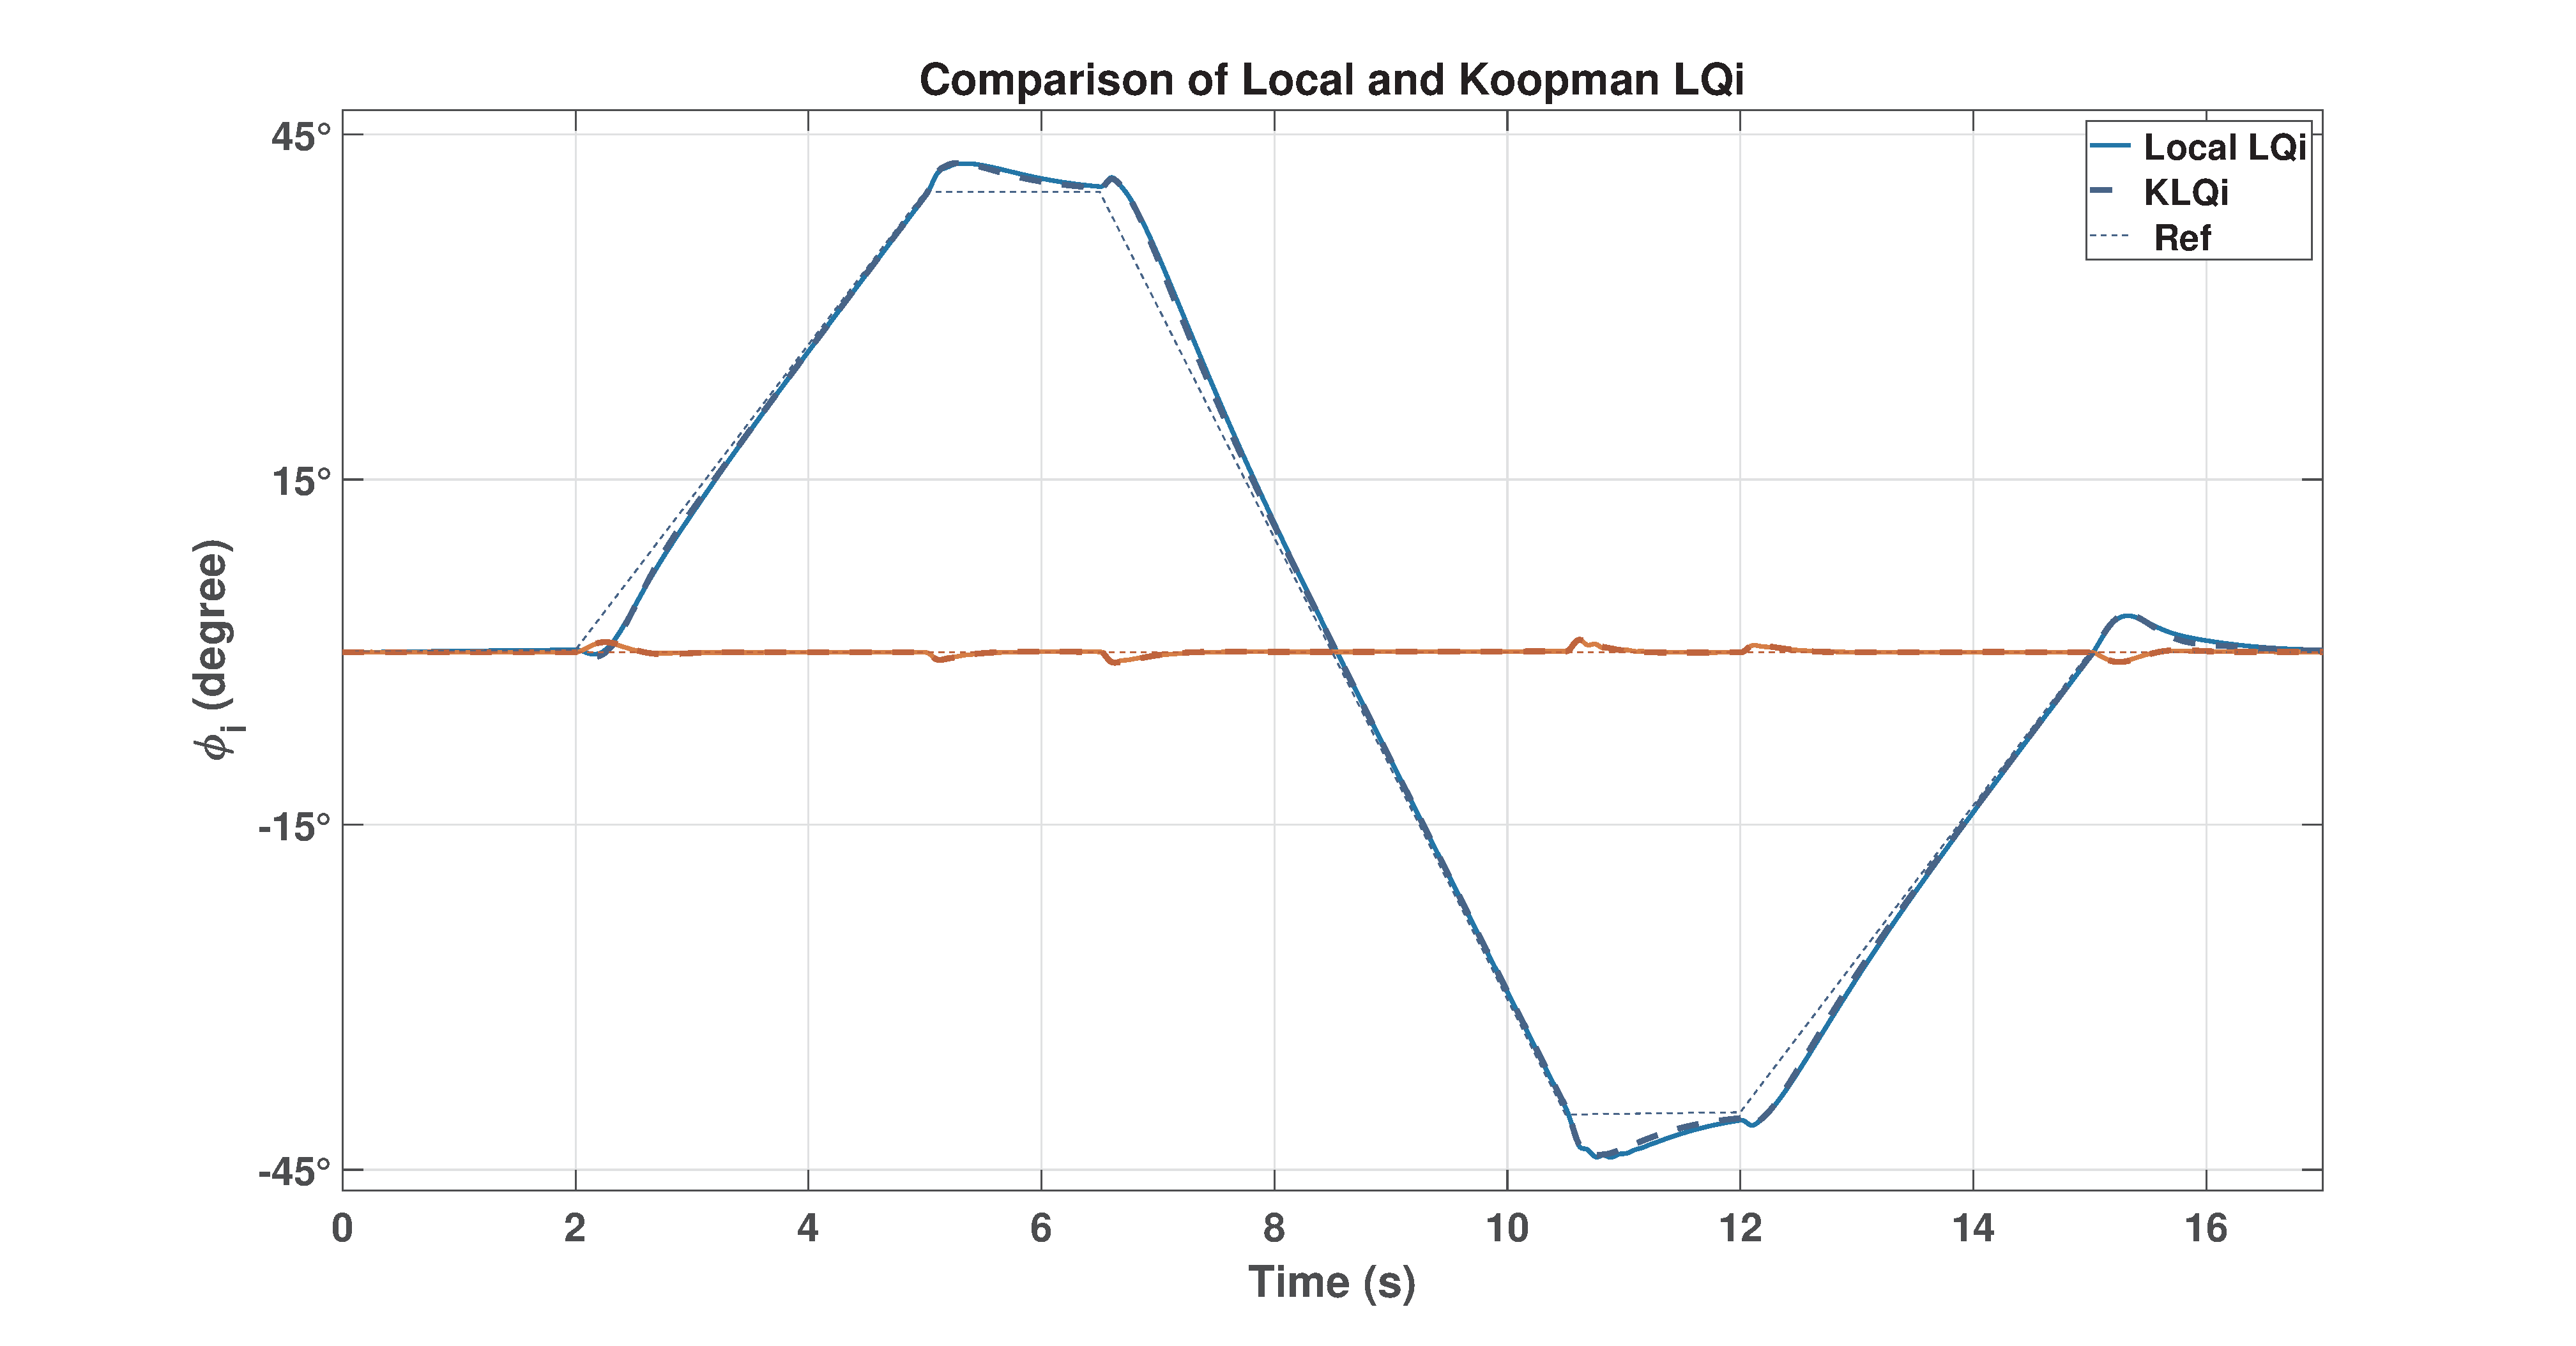
\includegraphics[width=1\linewidth]{figures/LQi_comp_5ms}
    \caption{Comparison of LQi applied to locally linearized model versus Koopman model with $\mathbf{\Psi_1}$}
    \label{fig: LQi_comp}
\end{figure}
% 
\begin{figure}[H]
    \centering
    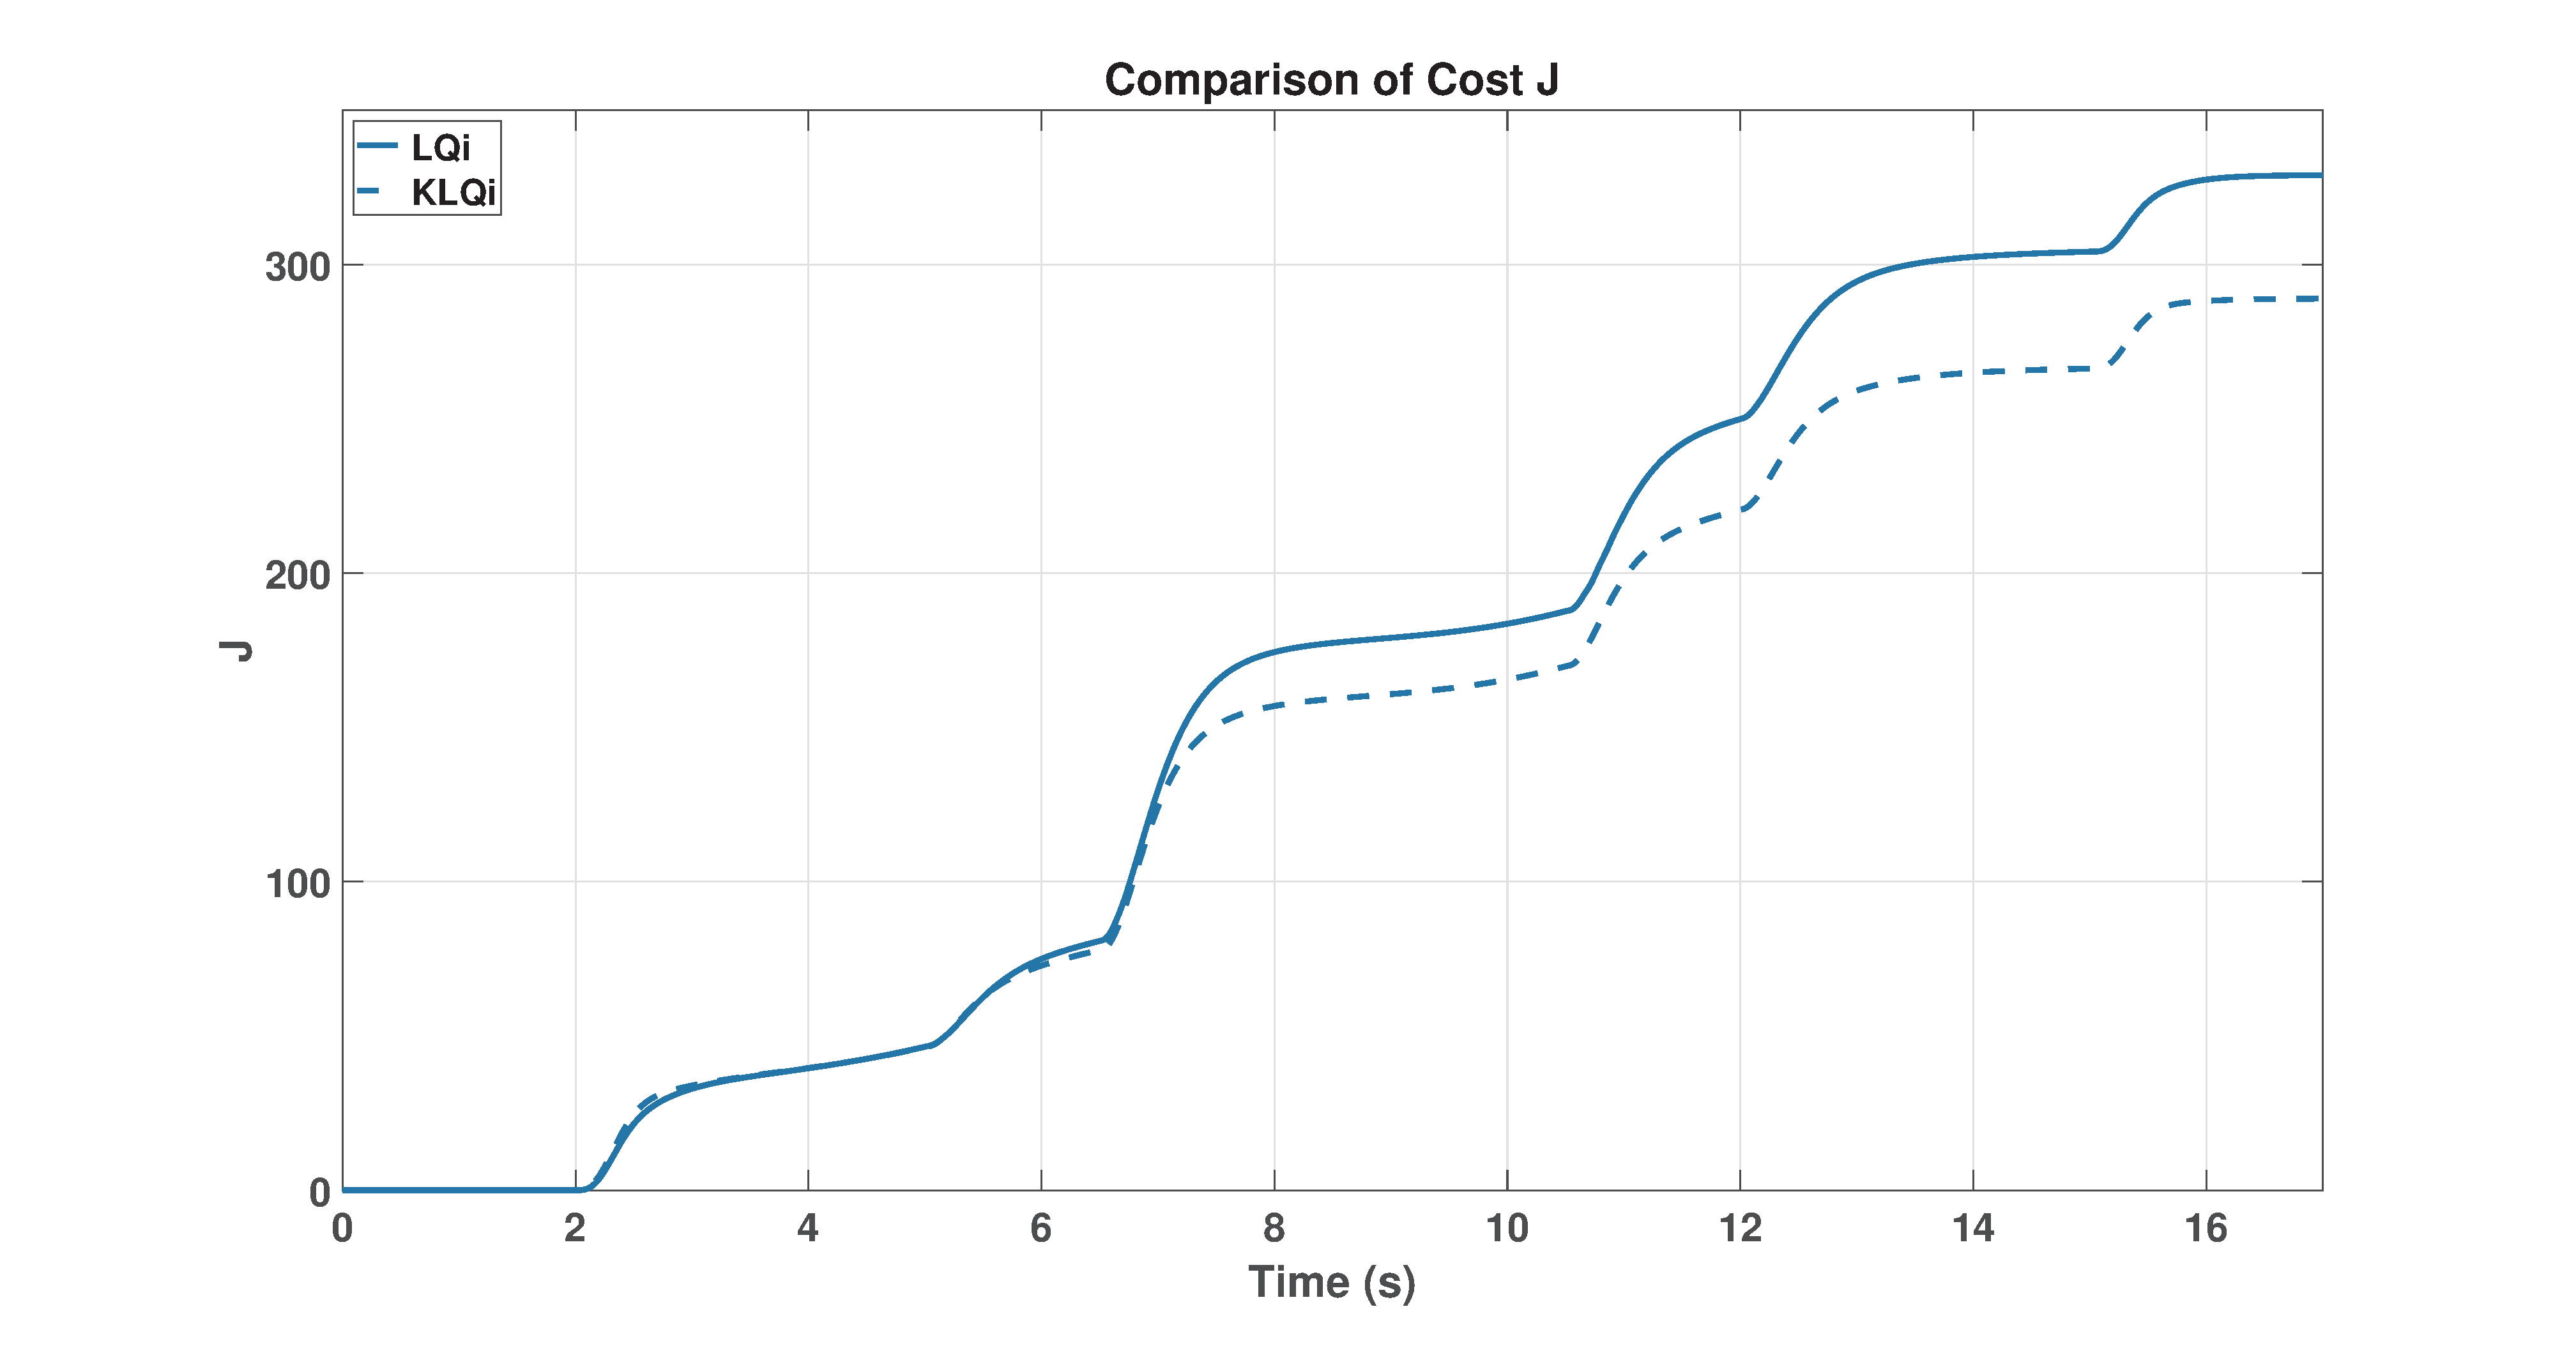
\includegraphics[width=1\linewidth]{figures/CostsLQi_5ms}
    \caption{Comparison of quadratic cost function $J$ for closed-loop tracking with local and Koopman operator approximated model}
    \label{fig: LQi_cost}
\end{figure}
% 
Next, a model predictive controller with a prediction horizon of $N_p = 200$, i.e. a prediction of 1 second into the future, was designed for the above-generated models. It was observed that the range of tracking could be increased from $40^{\circ}$ to $45^{\circ}$. This was expected as MPC almost always performs better than the linear quadratic regulator, especially more so in tracking problems. This is because, as opposed to the optimization of the quadratic cost function over an infinite time horizon as is the case with LQR (\ref{eq:Costfunc}), the MPC optimizes the cost function over a finite time horizon (\ref{eq:MPCcostfunction}) and repeatedly computes the optimal input. As a result, the controller can generate optimal control inputs valid for only a small fixed horizon instead of optimal control inputs that are valid over a very long period of time as in the case of a linear quadratic regulator. However, this comes at a cost. The optimal LQR input is computed offline and does not change during the process. In contrast, in MPC, the optimal input is computed online and, therefore, depends on the computer's computational capabilities. This cost can, however, be greatly reduced by formulating the MPC problem in a dense form (Eqs. \ref{eq:NstepComp} and \ref{eq:MPCdense}) as proposed by Korda et al. \cite{MPC_Korda}. The matrices $\mathbf{\Bar{A}}$ and $\mathbf{\Bar{B}}$ can be pre-computed offline, and one only needs to update the current state vector $\mathbf{x}_k$ online. This greatly reduces the computational effort and renders the MPC as feasible as the LQi in terms of implementation. Moreover, this dense formulation (Eq. \ref{eq:MPCdense}) is independent of the state's dimension and therefore, augmenting a state with nonlinear observables does not significantly affect the computational time of the MPC.  Figure \ref{fig: MPC_all} compares the local model's tracking performance against the Koopman model. Again, the overall quadratic cost functions are similar for local and Koopman models.
% 
\begin{figure}[H]
    \centering
    \includegraphics[width=1\linewidth]{figures/MPC_all_5ms}
    \caption{Comparison of MPC applied to local model versus Koopman model with $\mathbf{\Psi_1}$}
    \label{fig: MPC_all}
\end{figure}
% 
Table~\ref{tab:Exec_1} presents the corresponding computation times for the local and Koopman models executed with a sampling time of 5ms and 10ms. It should be noted that the controllers for the models generated from data sampled every 10ms are different from the controllers tuned for models generated from data sampled every 5ms. Both the controllers were GA-tuned to de-emphasize the effect of human bias. The comparison between the sampling times is made to highlight the trade-off between computation time and the model-controller combinations' performance. Table~\ref{tab:RMSE_1} presents the relative root-mean-square-error (in \% error w.r.t the reference trajectory of $\phi_1$) for the model-controller combinations explored until now in this section.
% 
\begin{table}[H]
    \centering
    \begin{tabular}{lcc}
         \toprule
                                  & \multicolumn{2}{c}{Average execution time~(ms)}\\
        \cmidrule{2-3}
         Model - Controller       & $T_s = 5$ms  & $T_s = 10$ms\\
         \midrule
         Local - MPC               & 0.56        & 0.17\\
         $\textup{KO}_1$ - MPC    & 0.59         & 0.18\\
         \bottomrule
    \end{tabular}
    \caption{Average execution time~(ms) of the MPC algorithms for different sampling times}
    \label{tab:Exec_1}
\end{table}
% 
\begin{table}[H]
    \centering
    \begin{tabular}{lcc}
         \toprule
                                            & \multicolumn{2}{c}{RMSE(\%)}\\
        \cmidrule{2-3}
         Model - Controller                  & $T_s = 5$ms & $T_s = 10$ms\\
         \midrule
         Local - LQi                         & 6.60       & 7.13\\
         $\textup{KO}_1$ - LQi               & 6.32       & 6.59 \\
         Local - MPC                         & 0.69       & 2.84\\
         $\textup{KO}_1$ - MPC               & 0.53       & 3.53\\
         \bottomrule
    \end{tabular}
    \caption{RMSE(\%) of tracking errors for different sampling times}
    \label{tab:RMSE_1}
\end{table}
% 
As observed in Section \ref{sec:Results_ident}, the choice of observables also plays an important role in approximating the system's dynamics farther away from the point of linearization. While there is no rule book which exactly governs the selection of such observables, it is often possible to work with proven basis functions used to approximate nonlinear dynamics in general. The only issue is that this space of observables spans infinite dimensions and therefore, one may or may not find the `correct' observables, which will serve the purpose. It is also important to note that not all nonlinear functions of the state approximate the Koopman operator. Some `observables' may even corrupt the system and/or drive the system to instability. Examples of such approximations are given in Kaiser et al. \cite{kaiser2020datadriven}. The choice of observables, therefore, is particular to the system of interest. In this thesis, the state was augmented with radial basis functions with randomly chosen centres as previously explained in Chapter \ref{Chapter:Data}. Figure~\ref{fig: LocalKMPC12} compares the performance of an MPC controller acting on the local model, a data-driven model approximated with 4 observables ($\mathbf{\Psi}_1$) that are simply the measurements of the state and another data-driven model with the state vector augmented by 50 radial basis functions ($\mathbf{\Psi}_4$, refer Sec. \ref{Chapter:Data}), respectively to track a reference trajectory of up to $45^\circ$. \par
Furthermore, it was observed that the range of tracking with MPC applied to the data-driven model approximated with an augmented vector of RBFs could be extended to almost $60^{\circ}$. Figure \ref{fig: KPMC_comp} compares the MPC controller designed for a Koopman model approximated with observables vector $\mathbf{\Psi}_1$, which could only track a reference trajectory as good as the local model (w.r.t the range), against a Koopman model approximated with the observables vector $\mathbf{\Psi}_4$ which could extend the range of tracking by almost $50\%$ for a wise choice of observables. As a result, one may hypothesize that there may exist a set of observables that could further extend the tracking range. An efficient way of arriving at such observables, however, is left to further research.
% 
\begin{figure}[H]
    \centering
    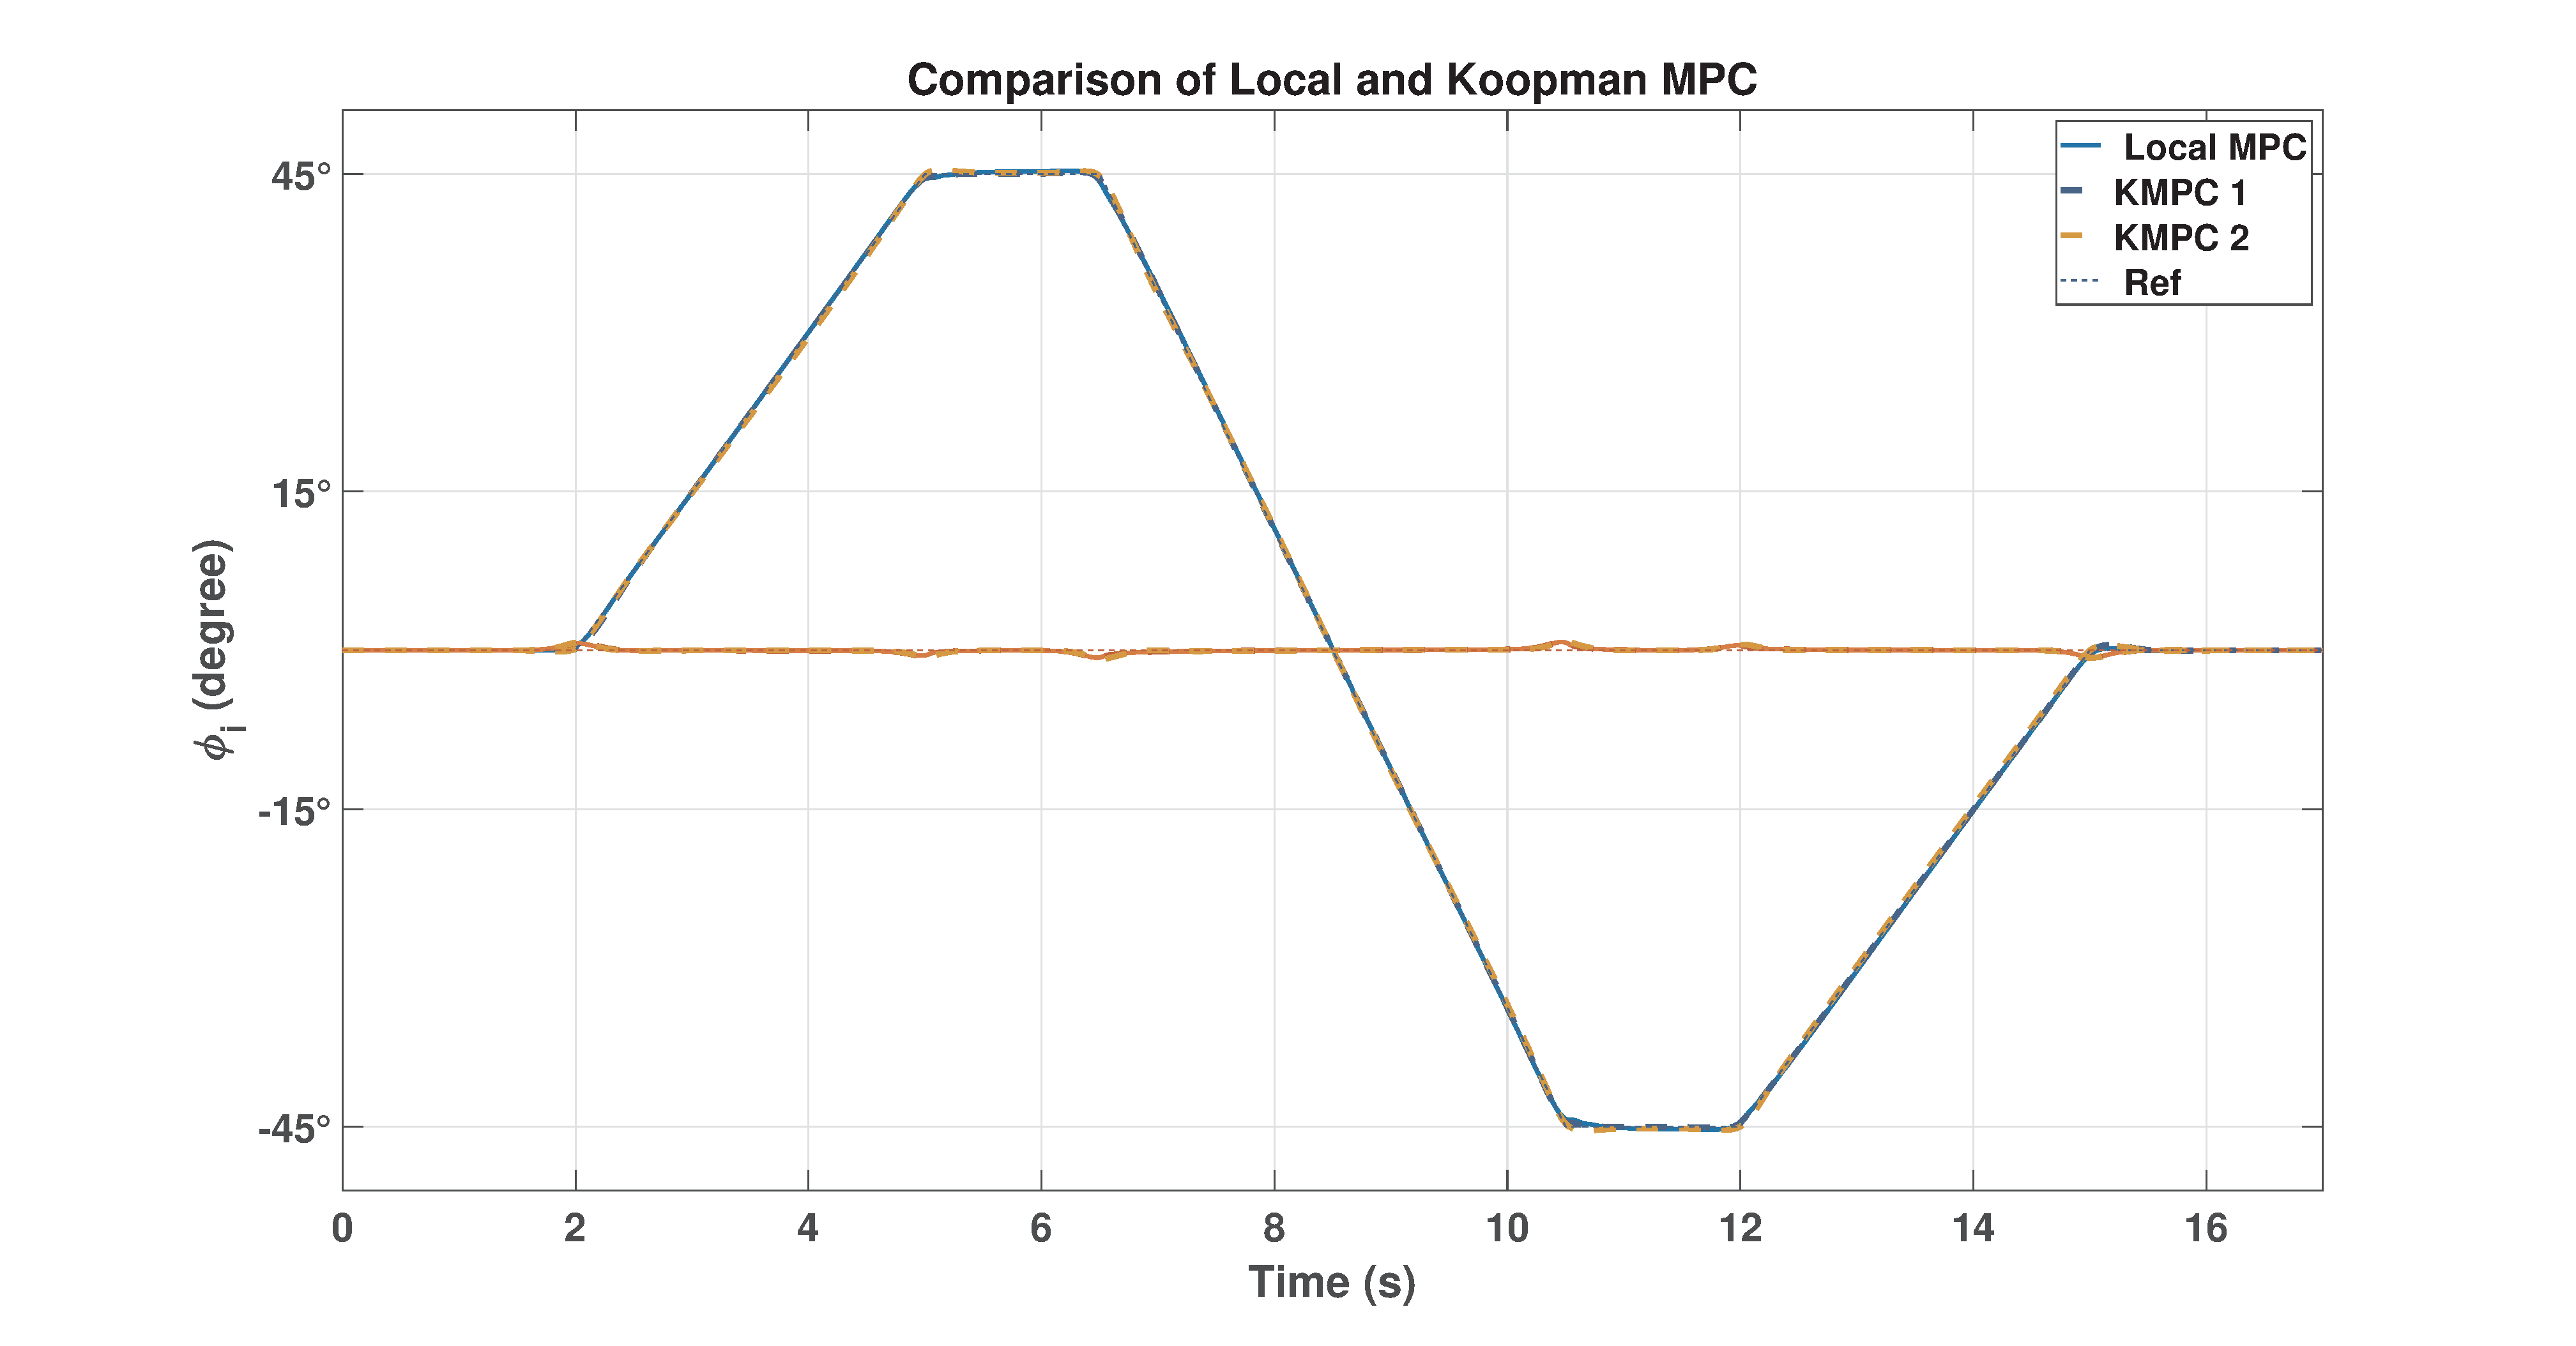
\includegraphics[width=1\linewidth]{figures/LocalKMPC12_5ms}
    \caption{Comparison of Local MPC, Koopman MPC for $\mathbf{\Psi_1}$ (KMPC1) and $\mathbf{\Psi}_4$} (KMPC2)
    \label{fig: LocalKMPC12}
\end{figure}
% 
% 
\begin{figure}[H]
    \centering
    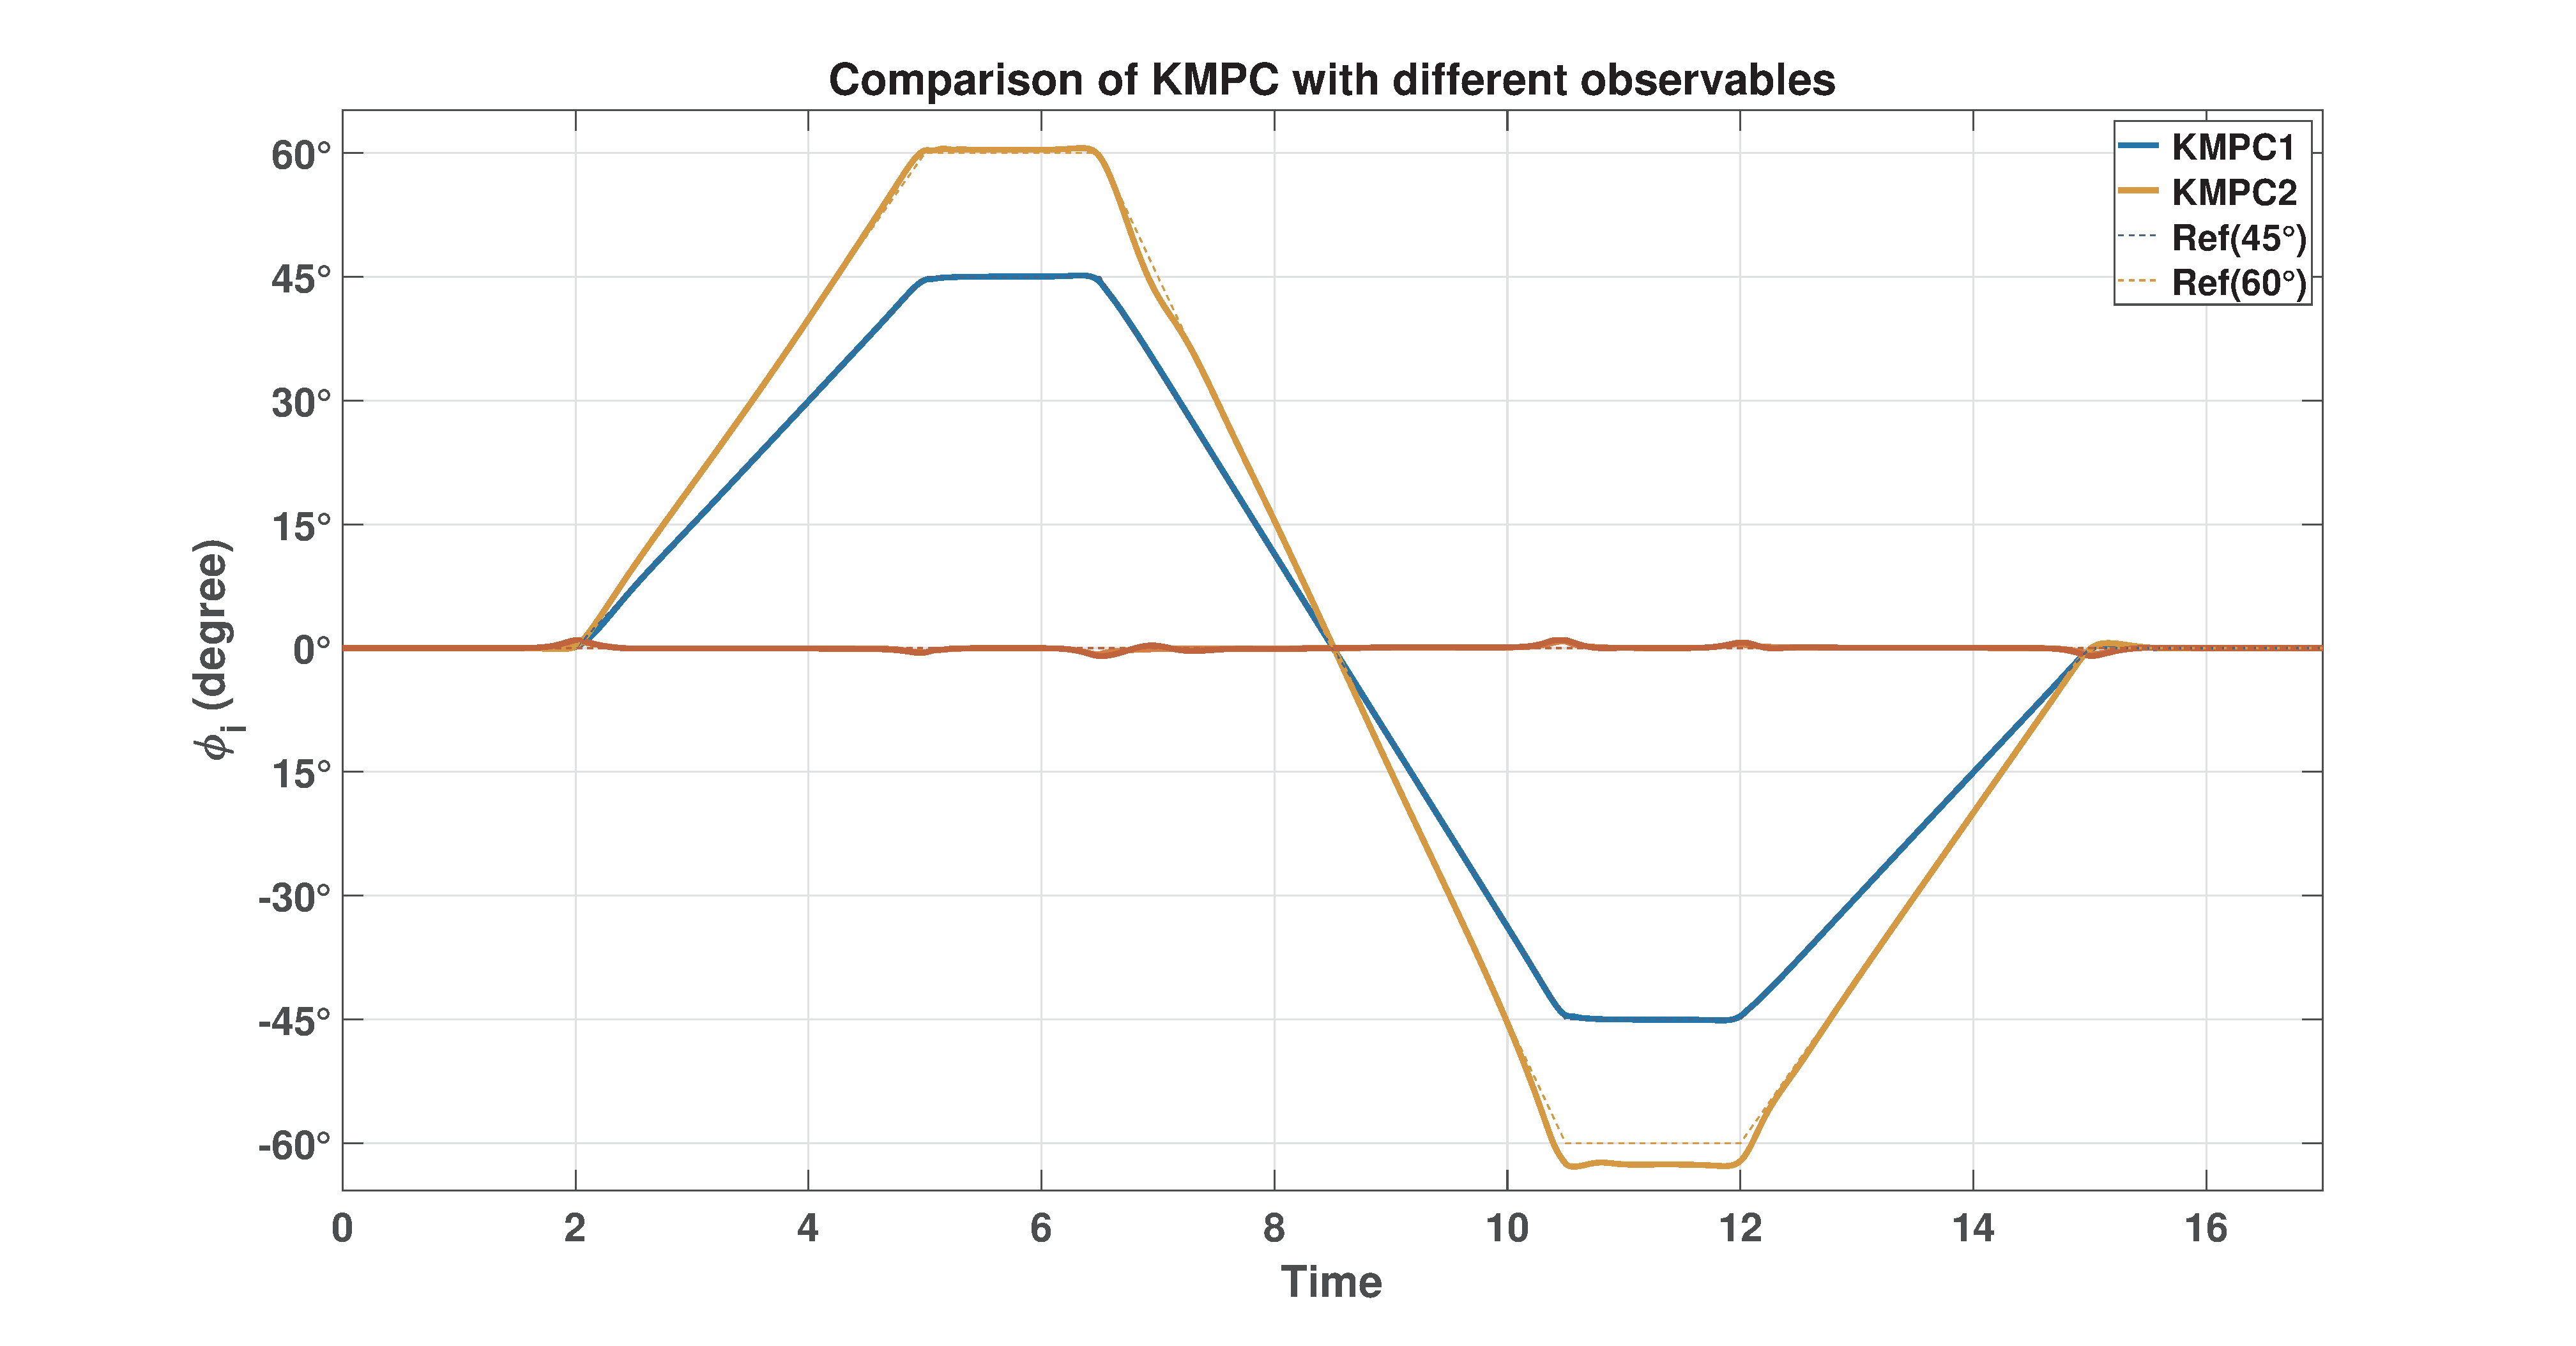
\includegraphics[width=1\linewidth]{figures/KMPC_comp_5ms}
    \caption{Comparison of Koopman MPC for $\mathbf{\Psi_1}$ (KMPC~1) and $\mathbf{\Psi}_4$} (KMPC~2)
    \label{fig: KPMC_comp}
\end{figure}
% 
Table~\ref{tab:Exec} and Table~\ref{tab:RMSE_2} compare the average execution times and relative RMSE for the above presented model-controller combinations, respectively. It can be seen that while the range of tracking could successfully be increased from $45^\circ$ to $60^\circ$ by augmenting the state vector with RBFs, there is no significant increase in the computation time or the relative RMSE (for $45^\circ$ reference trajectory). This is due to the dense formulation of the MPC, as discussed previously. The slight increase in computation time is because one needs to lift the system's state at every computation step. However, the augmented state would have a negligible effect on the computation time of the optimal control input as the matrices $\mathbf{\Bar{A}}$ and $\mathbf{\Bar{B}}$ are pre-computed offline. \par
In the following tables in this section, $\textup{KO}_1$ and $\textup{KO}_2$ are the data-driven models generated by the observables $\mathbf{\Psi}_1$ and $\mathbf{\Psi}_4$, respectively.
\begin{table}[H]
    \centering
    \begin{tabular}{lcc}
         \toprule
                                  & \multicolumn{2}{c}{Average execution time~(ms)}\\
        \cmidrule{2-3}
         Model - Controller       & $T_s = 5$ms  & $T_s = 10$ms\\
         \midrule
         Local - MPC               & 0.56        & 0.17\\
         $\textup{KO}_1$ - MPC    & 0.59         & 0.18\\
         $\textup{KO}_2$ - MPC    & 0.69         & 0.28\\
         \bottomrule
    \end{tabular}
    \caption{Average execution time~(ms) of the MPC algorithms for different sampling times}
    \label{tab:Exec}
\end{table}
% 
\begin{table}[H]
    \centering
    \begin{tabular}{lcc}
         \toprule
                                            & \multicolumn{2}{c}{RMSE(\%)}\\
        \cmidrule{2-3}
         Model - Controller                  & $T_s = 5$ms & $T_s = 10$ms\\
         \midrule
         Local - LQi                         & 6.60       & 7.13\\
         $\textup{KO}_1$ - LQi               & 6.32       & 6.59 \\
         Local - MPC                         & 0.69       & 2.84\\
         $\textup{KO}_1$ - MPC               & 0.53       & 3.53\\
         $\textup{KO}_2$ - MPC - $45^\circ$  & 0.72       & 3.49\\
         $\textup{KO}_2$ - MPC - $60^\circ$  & 2.67       & 2.45\\
         \bottomrule
    \end{tabular}
    \caption{RMSE(\%) of tracking errors for different sampling times}
    \label{tab:RMSE_2}
\end{table}
Next, the robustness of tracking is tested for the synthesized controller. Originally, the controller was synthesized (GA-tuned) for the trajectory shown in Fig.~\ref{fig:ReferenceTraj} where the time to reach the extreme points was $T = 3s$. It is interesting to observe this controller's behaviour on trajectories with steeper slopes, for example, with $T = 1.5s$ and $T = 1s$. Table~\ref{tab:RMSE_diffslopes} presents the results of such a comparison. The values shown in red correspond to the percentage increase in the relative RMSE to the relative RMSE of the model-controller combinations for the original reference trajectory, presented in the first column. It must be noted that from here on, the comparisons are made for data-driven models approximated with data sampled at 5ms. The reason 5ms was selected is that the computation times (Table~\ref{tab:Exec}) are well within the hardware capabilities of the computer and the relative RMSE (Table~\ref{tab:RMSE_2}) for $T_s = 5$ms is much lesser in all the cases when compared to $T_s = 10$ms, making the sampling time of 5ms an obvious choice.
\begin{table}[H]
    \centering
    \begin{tabular}{llll}
         \toprule
                                            & \multicolumn{3}{c}{RMSE(\%)}\\
        \cmidrule{2-4}
         Model - Controller                  & $T = 3$s & $T = 1.5$s & $T = 1$s \\
         \midrule
         Local - LQi                         & 7.13       & 10.03~(\textcolor{red}{+40.7\%})      & 13.35~(\textcolor{red}{+87.2\%})\\
         $\textup{KO}_1$ - LQi               & 6.59       & 9.26~(\textcolor{red}{+40.5\%})       & 12.55~(\textcolor{red}{+90.4\%})\\
         Local - MPC                         & 0.69       & 0.94~(\textcolor{red}{+36.2\%})       & 1.26~(\textcolor{red}{+82.6\%})\\
         $\textup{KO}_1$ - MPC               & 0.53       & 0.85~(\textcolor{red}{+60.3\%})       & 1.29~(\textcolor{red}{+143.4\%})\\
         $\textup{KO}_2$ - MPC - $45^\circ$  & 0.72       & 0.86~(\textcolor{red}{+19.4\%})       & 1.58~(\textcolor{red}{+119.4\%})\\
         $\textup{KO}_2$ - MPC               & 2.67       & 2.87~(\textcolor{red}{-})       & 2.67~(\textcolor{red}{-})\\
         \bottomrule
    \end{tabular}
    \caption{RMSE(\%) of tracking errors for different target times $T$}
    \label{tab:RMSE_diffslopes}
\end{table}
A few observations are in order. 
\begin{itemize}
    \item Firstly, consider the first two rows; it can be seen that the percentage increase in the relative RMSE for the local model and Koopman model $\textup{KO}_1$ is comparable, which means that the recorded data captured most of the dynamics of the underlying nonlinear dynamical system. This consequently validates the approach employed in Section~\ref{sec:Results_ident} to record the data and highlights the effectiveness of the data-driven regression methods described in Chapter~\ref{Chapter:Prelims}.
    \item Next, comparing rows 1 and 3 it can be seen that the MPC controller performs slightly better compared to the LQi, which is of course expected. Also, note that the relative RMSE was significantly lower for the MPC controller to start with.
    \item The comparison of rows 4 and 5 shows that the model with state vector augmented with RBFs seems to capture relatively more relevant dynamics than just the state vector as observables, and consequently, the relative increase in the RMSE for varying slopes is much lesser, i.e., the model-controller combination, ($\textup{KO}_2 - \textup{MPC}$), seems to track the various trajectories much closer than the $\textup{KO}_1 - \textup{MPC}$ combination.
    \item It is seen that the result of comparison between row 2 and row 4, LQi and MPC controller applied to the $\textup{KO}_1$ model, respectively, is not as expected. The MPC controller performs relatively worse than an LQi controller. A possible explanation for this could not be ascertained. It could only be guessed that the $\textup{KO}_1-\textup{MPC}$ combination has the lowest relative RMSE of all the combinations for $T = 3s$, and a small but reasonable increase in the RMSE contributes much more than compared to the same in the case of KLQi.
    \item The last row presents some important insight into the choice of observables.\\Figure~\ref{fig: cont_traj} visualizes the results of the last row. It can be seen that as the slope becomes steeper, the tracking range of the model-controller combination decreases. A potential explanation to this could be that the choice of observables, while good, may not be the best, and there may exist some other combination of RBFs which perform better. This is left to further research. It can also be construed as a possible limitation of data-driven models, and that these models may not perform as well as a model derived from first principles. This can be seen in the following results. 
\end{itemize}
% 
\begin{figure}[H]
    \centering
    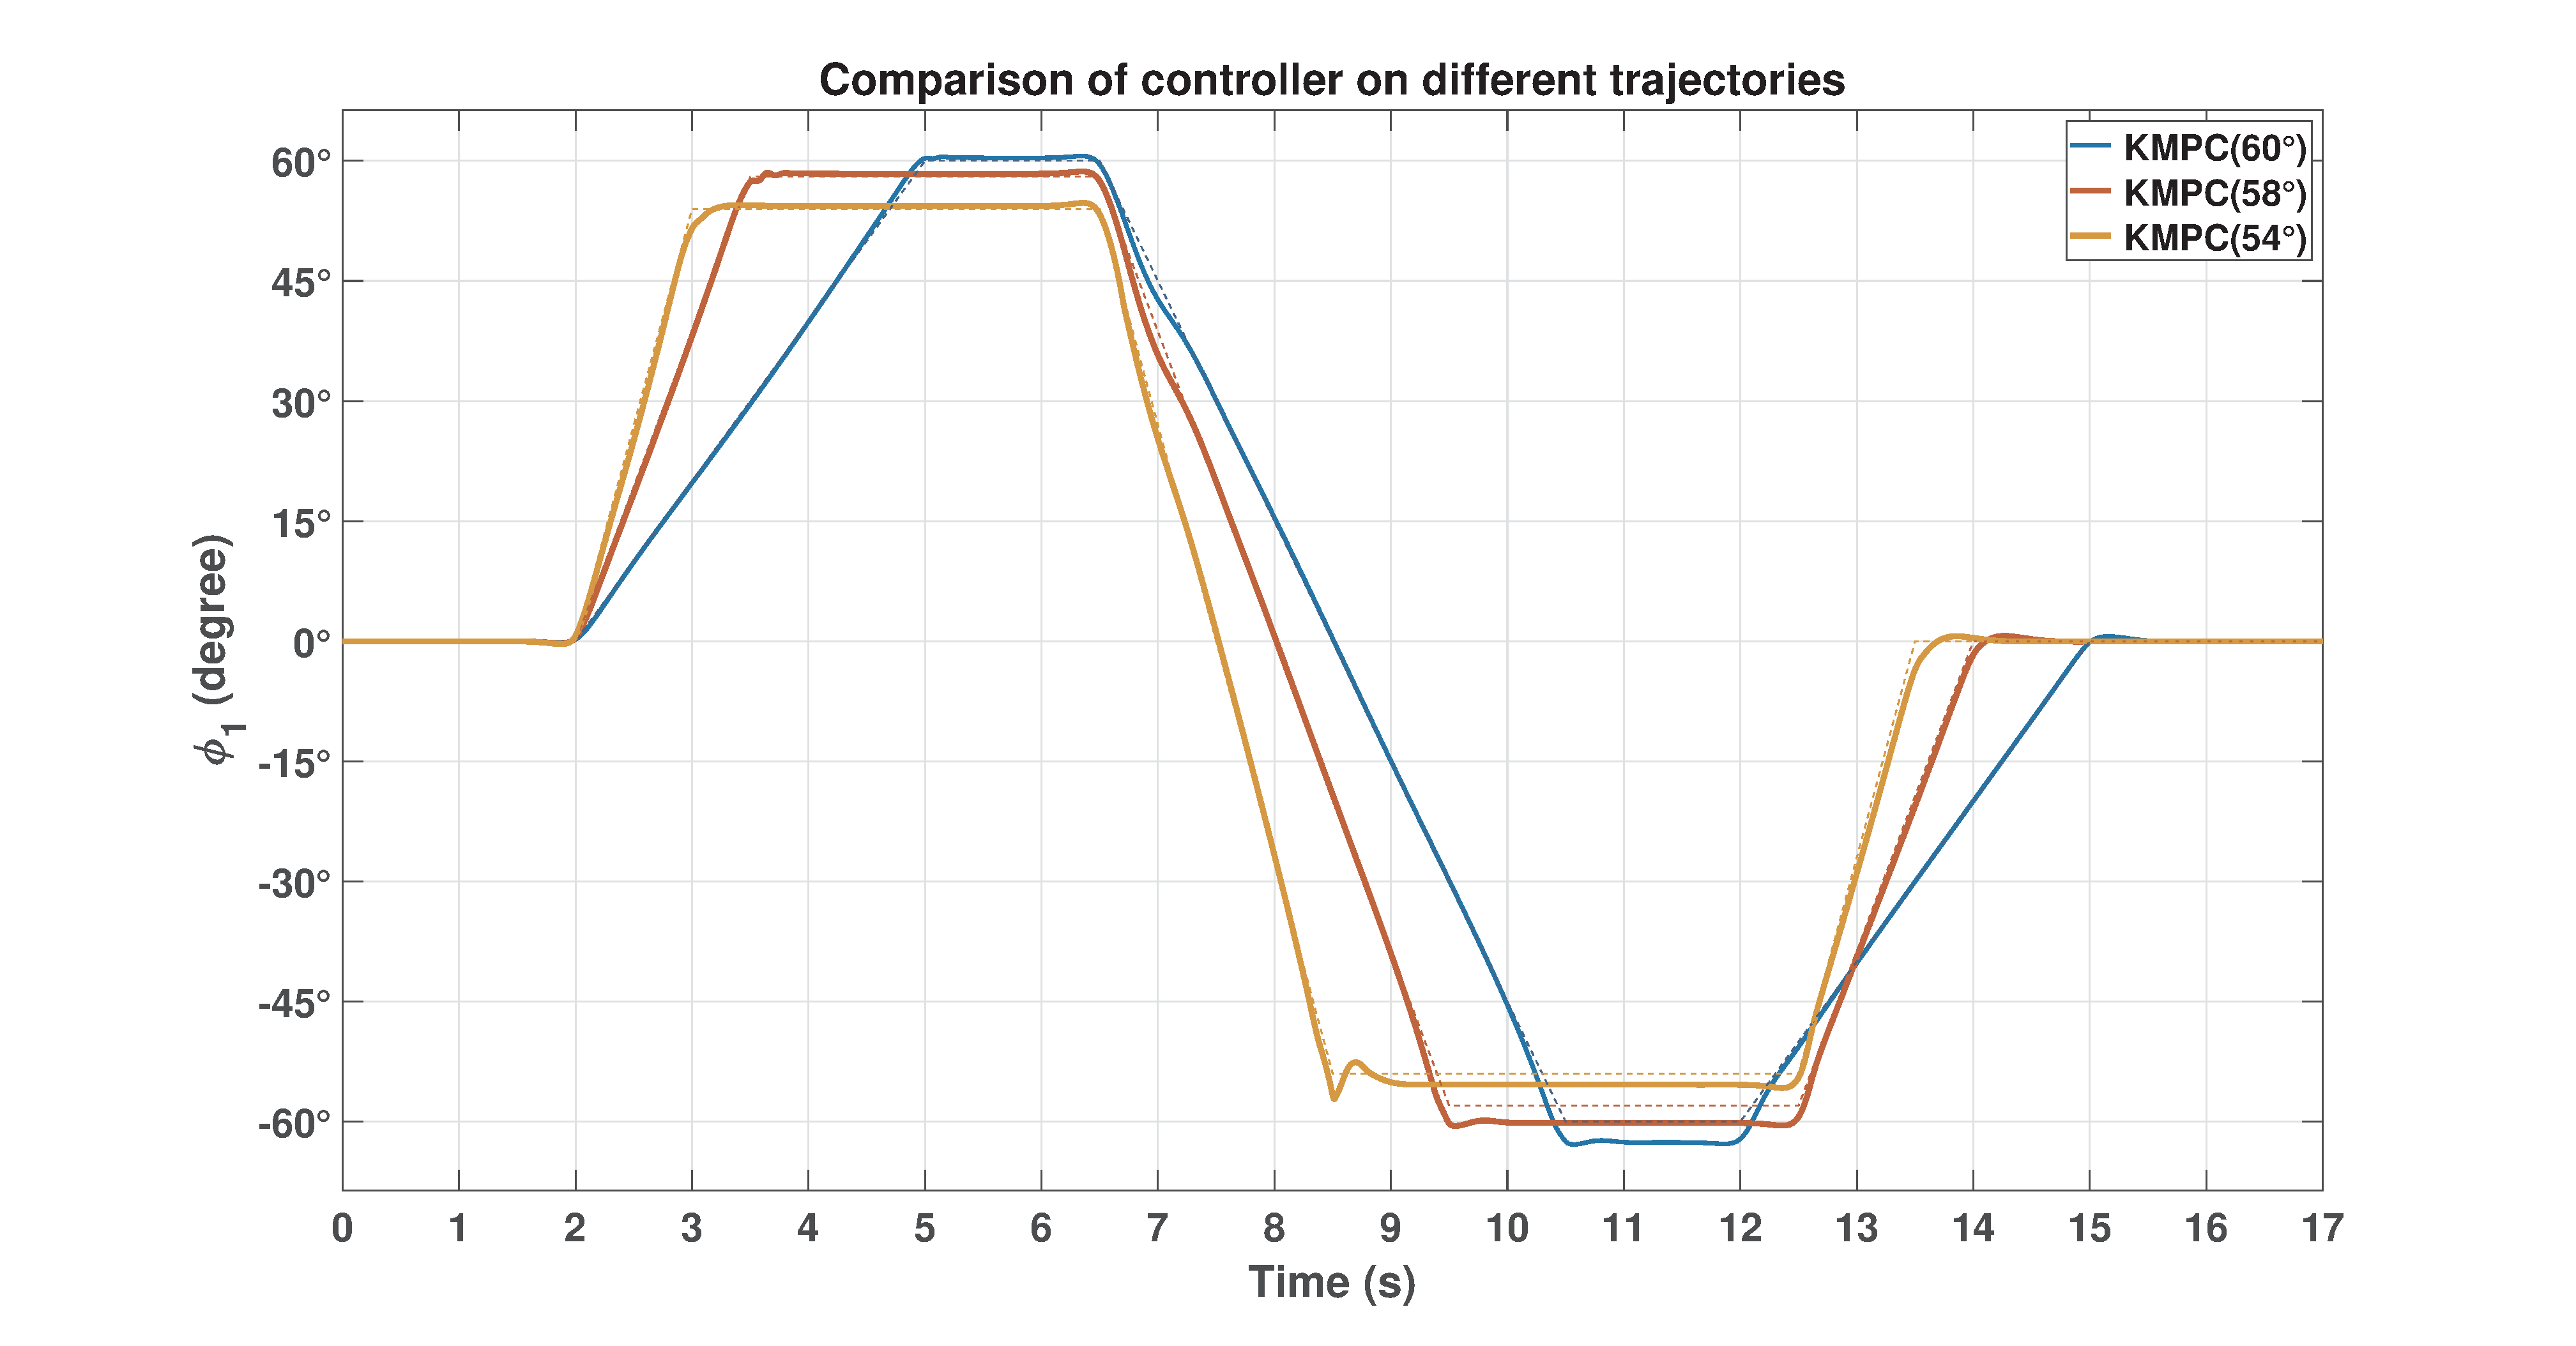
\includegraphics[width=1\linewidth]{figures/Cont_diffTraj}
    \caption{Comparison of the synthesized controller on reference trajectories with different degrees of slopes for Koopman model approximated using $\mathbf{\Psi}_4$. (\textcolor{blue}{\textbf{--}}) -- $T = 3s$,(\textcolor{red}{\textbf{--}}) -- $T = 1.5s$, and (\textcolor{orange}{\textbf{--}}) -- $T = 1s$}
    \label{fig: cont_traj}
\end{figure}
% 
Consider a quasi-linear parameter varying~(qLPV) model of the ADIP parameterized with scheduling parameters $\rho = [\phi_1 \quad \Dot{\phi}_1]$ as described by Cisneros et al. \cite{qLMPC}. A corresponding MPC controller is synthesized for this model, tuned by a GA. The tuning parameters are $\mathbf{Q} = \textup{diag}(1884.43,~1777.43,~80.16,~0.76)$ and $\textup{R} = 26.13$ and $\mathbf{Q}_N = 2219.42\mathbf{Q}$.\par
It is important to note that the prediction horizon for the qLPV-MPC (here-on, qLMPC) is taken as $N_p = 40$, as against $N_p = 200$, which was the prediction horizon considered previously. The reason to choose a lower prediction horizon in the case of qLMPC is that, at every time step, a linear model is computed for which a new MPC is synthesized which then returns the optimal control input for the next time step and this process is repeated. This is a computationally costly process, and the computation cost further increases exponentially with the increase in the prediction horizon. Table~\ref{tab:Exec_predHor} illustrates this. 
\begin{table}[H]
    \centering
    \begin{tabular}{lcc}
         \toprule
                                  & \multicolumn{2}{c}{Average execution time~(ms) for $T_s$ = 5ms}\\
        \cmidrule{2-3}
         Model - Controller       & $N_p = 200$  & $N_p = 40$\\
         \midrule
         Local - MPC               & 0.56        & 0.05\\
         $\textup{KO}_1$ - MPC    & 0.59         & 0.06\\
         $\textup{KO}_2$ - MPC    & 0.69         & 0.16\\
         $\textup{qLPMC}$         & 10.2         & 0.40\\
         \bottomrule
    \end{tabular}
    \caption{Average execution time~(ms) of the MPC algorithms for different prediction horizons}
    \label{tab:Exec_predHor}
\end{table}
It can be seen that for a prediction horizon of $N_p = 200$, the computation time is more than 10ms for the qLMPC, whereas it is 0.40ms for a prediction horizon of $N_p = 40.$ Moreover, the results obtained with $N_p = 40$ can be considered good enough, and there is actually no need to increase the prediction horizon further. In previously considered models, however, the possibility of a longer prediction horizon enables better results. One can use the prediction horizon of $N_p = 200$, simply because the computational cost is well within the hardware requirements. The corresponding results are quite good. The average execution time of the MPC for the local model and data-driven model is significantly low even with a prediction horizon of $N_p = 200$ because the MPC here is based on a linear model whose matrices are pre-computed offline as against online computation of the linear matrices in the case of qLMPC. \par
Figure~\ref{fig: cont_traj_qLMPC} presents a qLMPC version of the comparison made previously in Fig.~\ref{fig: cont_traj}. 
% 
\begin{figure}[H]
    \centering
    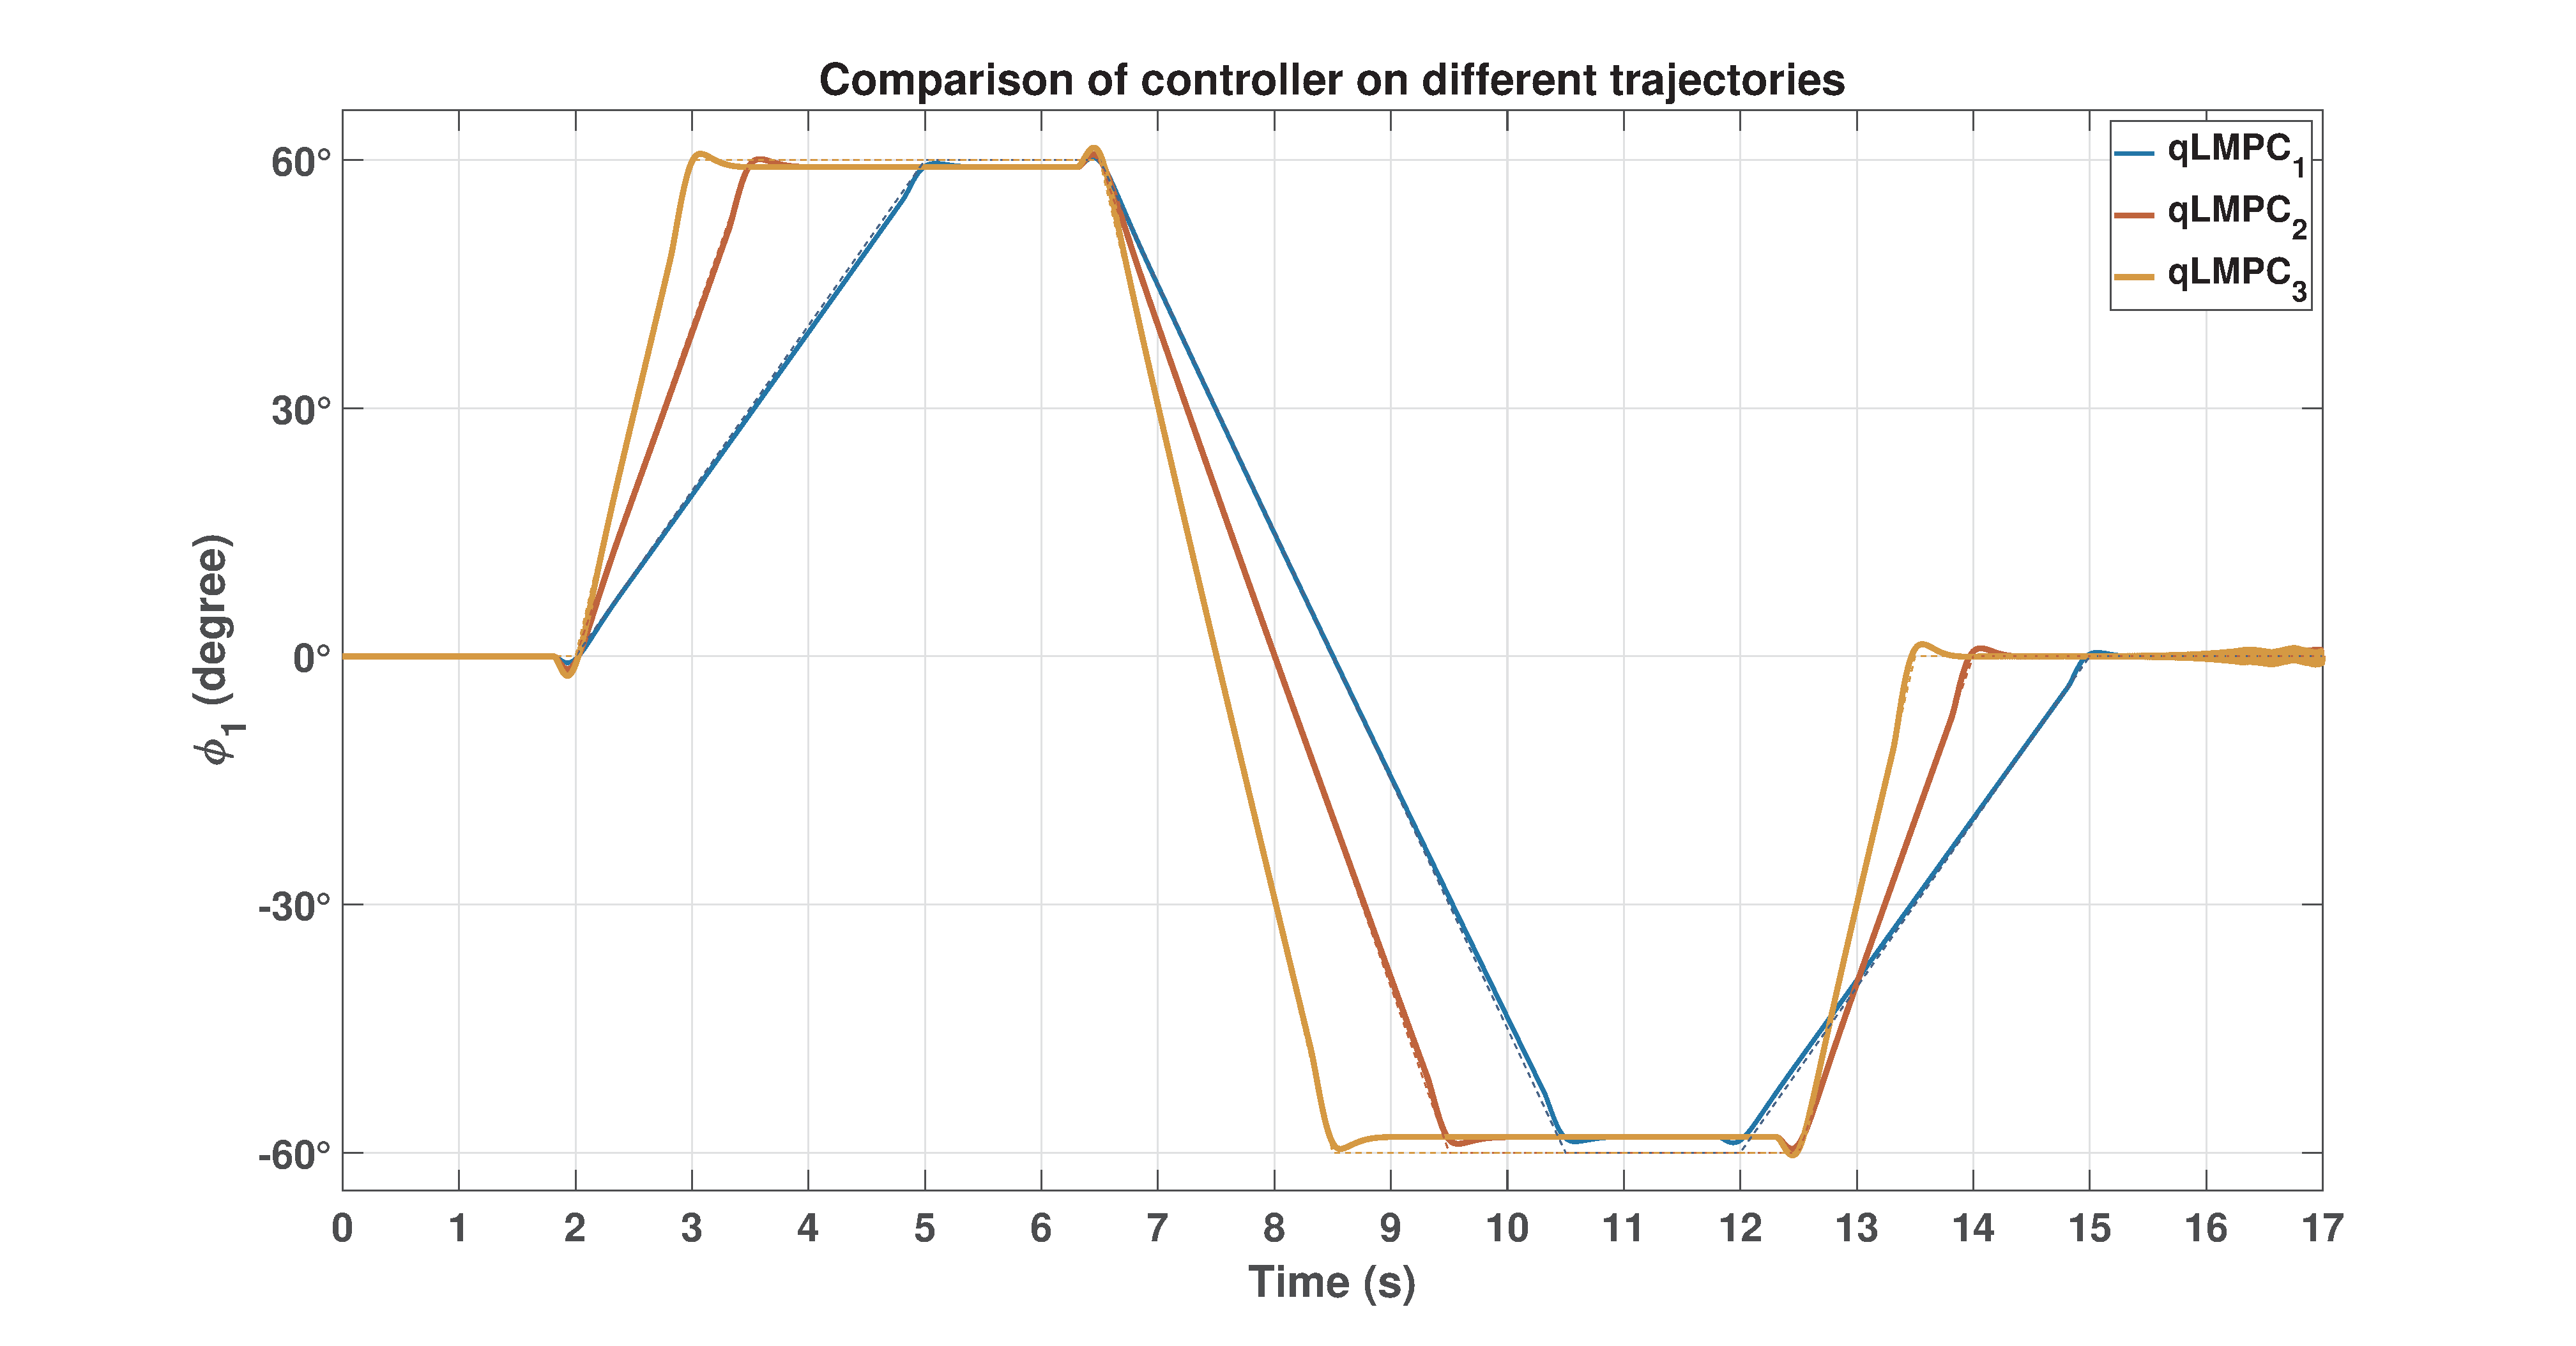
\includegraphics[width=1\linewidth]{figures/qLMPC_comp}
    \caption{Comparison of the synthesized qLMPC controller on reference trajectories with different degrees of slopes. (\textcolor{blue}{\textbf{--}}) -- $T = 3s$,(\textcolor{red}{\textbf{--}}) -- $T = 1.5s$, and (\textcolor{orange}{\textbf{--}}) -- $T = 1s$}
    \label{fig: cont_traj_qLMPC}
\end{figure}
% 
The corresponding relative RMSE values are presented in Table~\ref{tab:RMSE_diffslopes_qlmpc}.
\begin{table}[H]
    \centering
    \begin{tabular}{lccc}
         \toprule
                                            & \multicolumn{3}{c}{RMSE(\%)}\\
        \cmidrule{2-4}
         Model - Controller                  & $T = 3$s & $T = 1.5$s & $T = 1$s \\
         \midrule
         qLPV - MPC                         & 2.15       & 2.24     & 2.43\\
         \bottomrule
    \end{tabular}
    \caption{RMSE(\%) of tracking errors for different target times}
    \label{tab:RMSE_diffslopes_qlmpc}
\end{table}
% 
An important observation can be made from Fig.~\ref{fig: cont_traj_qLMPC} and Table~\ref{tab:RMSE_diffslopes_qlmpc}; the relative RMSE does not increase significantly with change in the slope of the reference trajectory, and also, the RMSE for qLMPC is lesser than that of a data-driven model with MPC approximated with $\mathbf{\Psi}_4$. Furthermore, the qLMPC can track up to $60^\circ$ for all the degrees of slope considered whereas, the $\textup{KO}_2-\textup{MPC}$ failed to track the desired target for steeper slopes of the reference trajectory. This points out a key limitation of data-driven models. A data-driven model might work better than a locally linearized first-principles model in the region where training data is captured, but it is possible that the data models may not perform on par with a quasi-linear parameter varying model. With the increase in computational capabilities, the qLPV approach seems much more promising. Nevertheless, one must note that an important assumption made here is the availability of a mathematical model of the system. Without this, the qLPV approach is not possible and the data-driven model stands as the obvious choice. \par
During the course of implementation, two additional important observations were made. First, although the Koopman approximated system is a linear representation of the underlying nonlinear dynamics, and in theory one can use any of the model-based linear control techniques to control the system, it is highly recommended to use a predictive controller like the MPC rather than a non-predictive controller like LQi for tracking tasks. This is because the extended state of observables more often than not contains nonlinear functions of the state. The LQi which computes the cost over the infinite horizon fails to solve the optimal control problem. It requires careful handpicking of observables to overcome this. Whereas, since the MPC predicts only over a reasonably small time horizon, it is often easier to manage any irregularities caused by nonlinear observables' evolution. Therefore, when working with data-driven models, MPC is a better choice than non-predictive controllers.\par
Second, as an additional exercise, the possibility of identifying and controlling a highly unstable system like the ADIP itself in the absence of an optimal controller was explored. At the beginning of this chapter, it was assumed that a plant model was already available. Therefore, an optimal controller, such as the linear quadratic regulator could be synthesized. A Koopman approximated linear system could then be modelled and controlled from just the measured closed-loop data. In the absence of such a controller, one may synthesize a non-model based PID controller that may not have the optimal tuning parameters for it to cover the necessary range of the desired trajectory. It was observed that it is possible to extend this range by recursively applying the EDMD approximation on the obtained data to generate a new linear model at every step for which a powerful model-based controller could be designed and consequently extend the range.\par
As an example, assume that the measurement data could be recorded for only $5^\circ$ from the up-up configuration after which the controller fails to track, as opposed to data recorded for a range of $40^\circ$ with an LQi controller(as shown in Fig \ref{fig:ReferenceTraj}). DMD could then be applied to such data to generate a linear model. With a linear model's availability, one could synthesize a model-based linear controller like the LQi or MPC. It is also possible to generate GA optimized tuning parameters for maximum reach. In this particular case, the range of tracking could be extended by an additional $10^\circ$ with an MPC's help and with the original measured state as the observable vector. Data was then recorded from this new system with a range of $15^\circ$, and the same process was applied to extend the range at each step. Finally, it was observed that the closed-loop tracking performance of the model-controller($\textup{KO}_3$-MPC) combination so obtained was comparable to that obtained from original data with the observable vector $\mathbf{\Psi}_1$. Figure~\ref{fig:diffdata} and Table \ref{tab:RMSE_3} illustrate the tracking performance of such a model with the same controller as used previously with other models. The results can be significantly improved with a controller specifically tuned for this model. However, it failed to perform as well with the $\mathbf{\Psi}_4$, i.e., with the observable vector containing the state and previously defined thin-plate spline RBFs. A potential reason for this might be the RBFs' choice, and there could be some combination of RBFs that may result in better performance. This is left to future research.
% 
\begin{figure}[H]
    \centering
    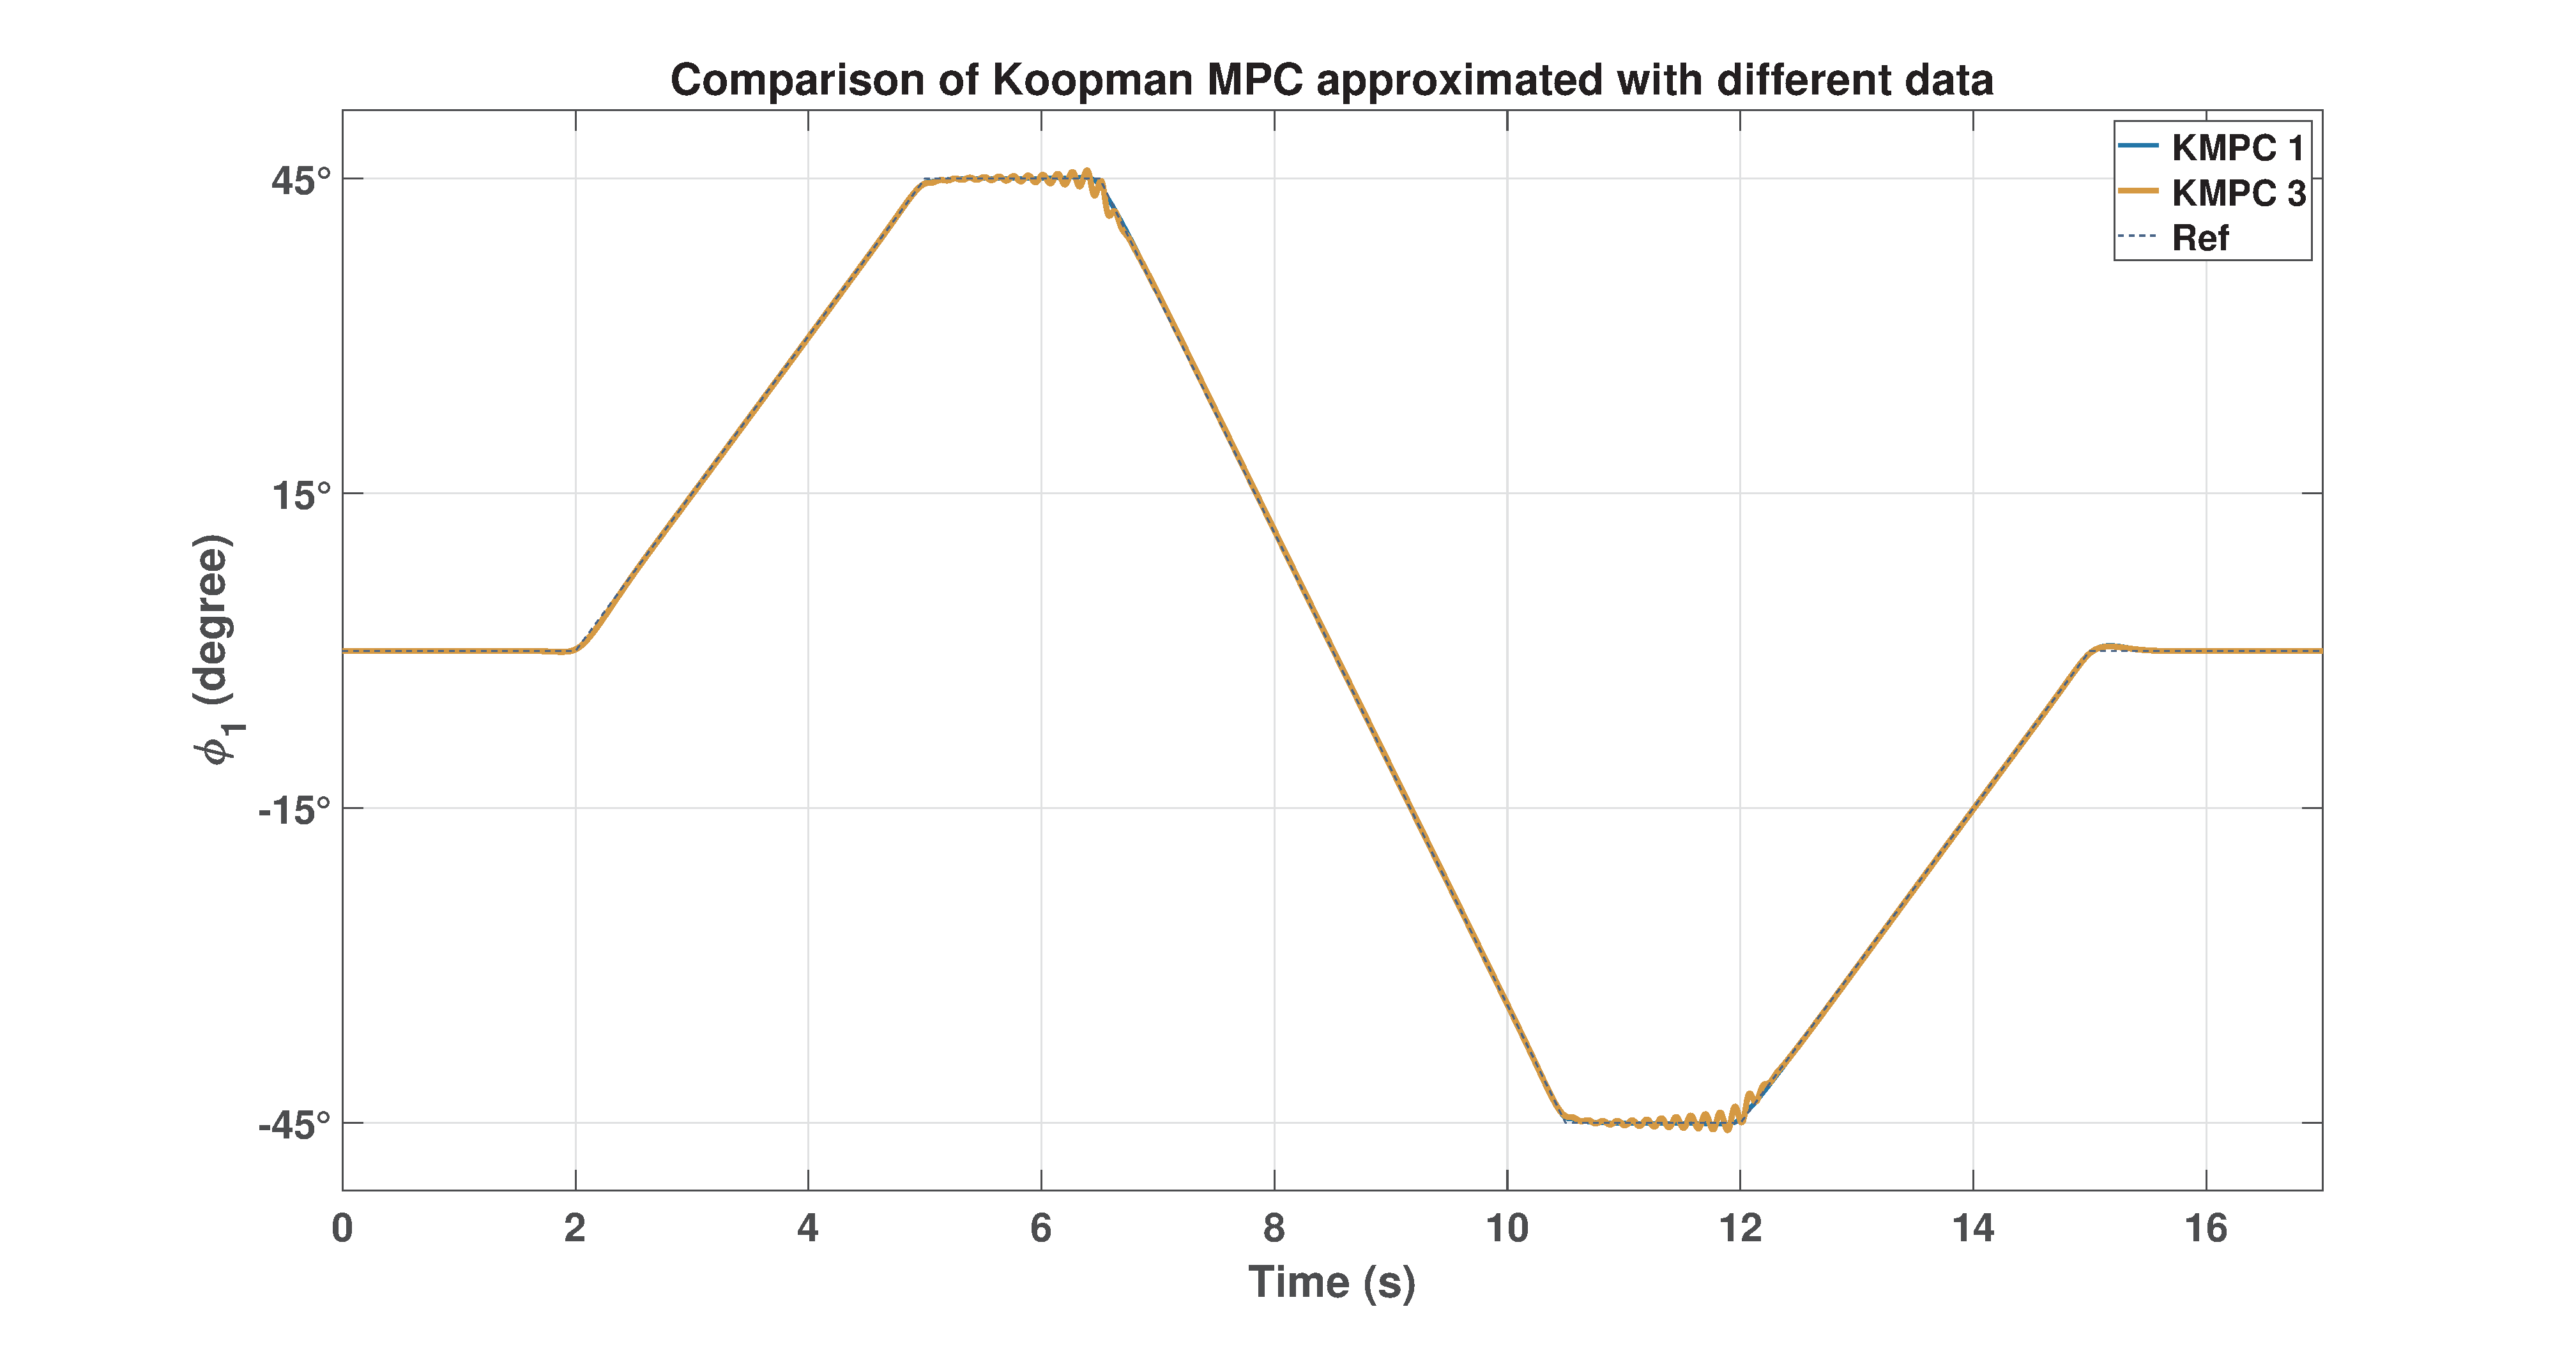
\includegraphics[width=1\linewidth]{figures/KMPC_diffdata}
    \caption{Comparison of Koopman MPC on data-driven model generated with data over a range of upto $40^\circ$ ($\textup{KO}_1$) versus data-driven model ($\textup{KO}_3$) constructed recursively with data generated over a range of upto $5^\circ$}
    \label{fig:diffdata}
\end{figure}
% 
% 
\vspace{-0.5cm}
\begin{table}[H]
    \centering
    \begin{tabular}{lc}
         \toprule
         Model - Controller                  & $T_s = 5$ms\\
         \midrule
         $\textup{KO}_1$ - MPC               & 0.53\\
         $\textup{KO}_3$ - MPC               & 0.95\\
         \bottomrule
    \end{tabular}
    \caption{RMSE(\%) of tracking errors for ($\textup{KO}_1$) and ($\textup{KO}_3$)}
    \label{tab:RMSE_3}
\end{table}
\vspace{-0.5cm}
It is important to reiterate two important assumptions made during the course of this implementation. First, the reference trajectories are fixed and are assumed to be known \textit{a priori}. This is important because the MPC controllers synthesized during the implementation are supplied with future values of the reference to enable the controller to `see' into the future and anticipate any changes in the trajectory. The controller then acts accordingly. This is different from the normally implemented MPC controllers, where only a current value of the reference is supplied. Figure~\ref{fig:antici} visualises this difference. When the controller is supplied with a reference signal of the next $N_p$ steps, it can anticipate the change in trajectory and respond accordingly. 
% 
\begin{figure}[H]
    \centering
    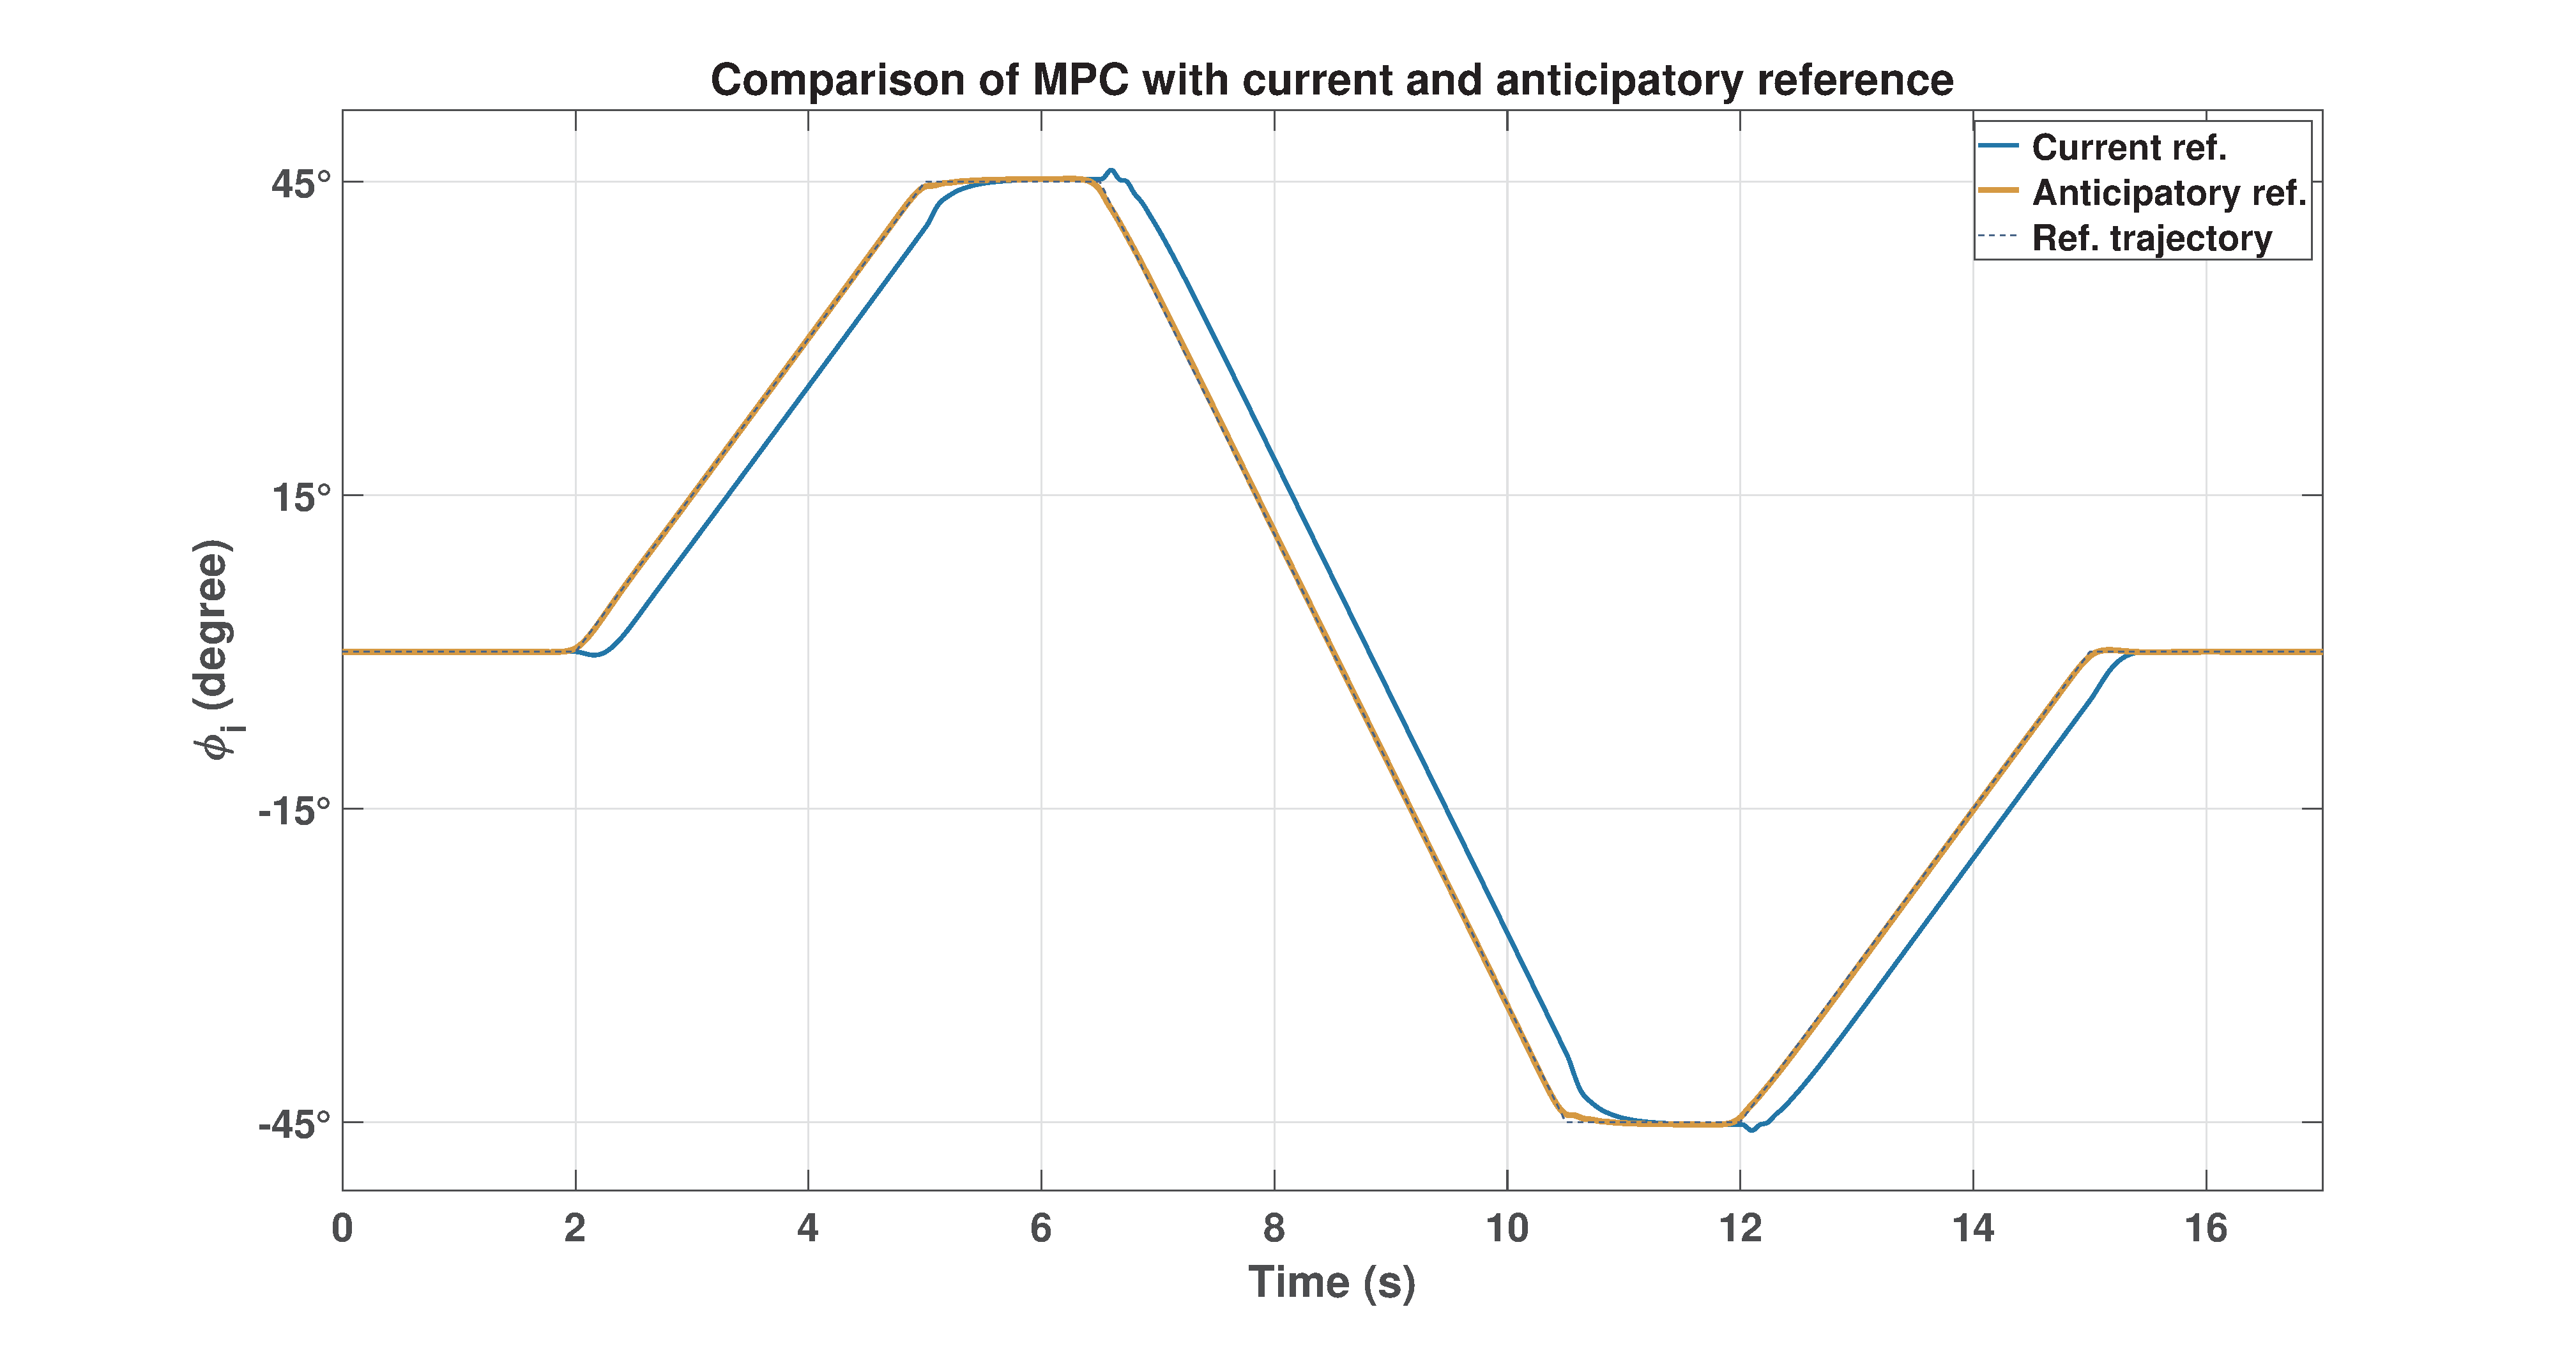
\includegraphics[width=1\linewidth]{figures/anticipatory}
    \caption{Comparison of controller acting on current reference versus anticipatory reference}
    \label{fig:antici}
\end{figure}
% 
\vspace{-0.55cm}
Second, a major assumption made during the genetic algorithm (GA) powered tuning of parameters in this thesis was that it was assumed a nonlinear simulation model of the plant (ADIP) is available to run the GA at all times. This may not always be the case, especially when dealing with systems where the dynamics are unknown. In such a case, one has to either resort to intuition and knowledge of tuning parameters or estimate a nonlinear black-box model of the unknown plant.
\vspace{-0.20cm}



